%%%%%%%%%%%%%%%%%%%%%%%%%%%%%%%%%%%%%%%%%%%%%%%%%%%%%%%%%%%%%%%%%%%
%%%%%%%%%%%%%%%%%%%%%%%%%%%%%%%%%%%%%%%%%%%%%%%%%%%%%%%%%%%%%%%%%%%

\documentclass[3p,times]{elsarticle}

%%%%%%%%%%%%%%%%%%%%%%%%%%%%%%%%%%%%%%%%%%%%%%%%%%%%%%%%%%%%%%%%%%%
%%%%%%%%%%%%%%%%%%%%%%%%%%%%%%%%%%%%%%%%%%%%%%%%%%%%%%%%%%%%%%%%%%%

%%%%%%%%%%%%%%%%%%%%%%%%%%%%%%%%%%%%%%%%%%%%%%%%%%%%%%%%%%%%%%%%%%%

\journal{Science of Computer Programming}

%%%%%%%%%%%%%%%%%%%%%%%%%%%%%%%%%%%%%%%%%%%%%%%%%%%%%%%%%%%%%%%%%%%

%%%%%%%%%%%%%%%%%%%%%%%
%% Elsevier bibliography styles
%%%%%%%%%%%%%%%%%%%%%%%
%% To change the style, put a % in front of the second line of the current style and
%% remove the % from the second line of the style you would like to use.
%%%%%%%%%%%%%%%%%%%%%%%

%% Numbered
%\bibliographystyle{model1-num-names}

%% Numbered without titles
%\bibliographystyle{model1a-num-names}

%% Harvard
%\bibliographystyle{model2-names.bst}\biboptions{authoryear}

%% Vancouver numbered
%\usepackage{numcompress}\bibliographystyle{model3-num-names}

%% Vancouver name/year
%\usepackage{numcompress}\bibliographystyle{model4-names}\biboptions{authoryear}

%% APA style
%\bibliographystyle{model5-names}\biboptions{authoryear}

%% AMA style
%\usepackage{numcompress}\bibliographystyle{model6-num-names}

%% `Elsevier LaTeX' style
\bibliographystyle{elsarticle-num}
%%%%%%%%%%%%%%%%%%%%%%%

\usepackage[cmex10]{amsmath}
\usepackage{amssymb}
\setcounter{tocdepth}{3}
\usepackage{graphicx}
%
\usepackage{url}
\urldef{\mailsa}\path|{peleska,huang}@uni-bremen.de|
\urldef{\mailsb}\path|ana.cavalcanti@york.ac.uk|
\urldef{\mailsc}\path|adenilso@icmc.usp.br|

\newcommand{\keywords}[1]{\par\addvspace\baselineskip
\noindent\keywordname\enspace\ignorespaces#1}

\usepackage{hyperref}

%\usepackage{float}
%\usepackage{lscape}
%\usepackage{lscape}
%
%\usepackage[linesnumbered,lined,boxed]{algorithm2e}
\usepackage[draft]{fixme}
%
\usepackage{zed-csp}
%
%\DeclareMathSymbol{\B}{\mathalpha}{AMSb}{"42}
%\DeclareMathSymbol{\I}{\mathalpha}{AMSb}{"49}
%\DeclareMathSymbol{\N}{\mathalpha}{AMSb}{"4E}
%\DeclareMathSymbol{\Pwr}{\mathalpha}{AMSb}{"50}
%\DeclareMathSymbol{\Q}{\mathalpha}{AMSb}{"51}
%\DeclareMathSymbol{\R}{\mathalpha}{AMSb}{"52}
%\DeclareMathSymbol{\Z}{\mathalpha}{AMSb}{"5A}
%\DeclareMathSymbol{\Sol}{\mathalpha}{AMSb}{"53}
%
%\newcommand{\obsv}[1]{{\cal O}(#1)}
%\newcommand{\ctrl}[1]{{\cal C}(#1)}
%\newcommand{\vdot}[1]{\stackrel{.}{#1}}
%
%\newcommand{\HS}{{\mathcal H}}
%
%\newcommand{\Interval}{\I}
%
\newcommand{\ist}{\mbox{{\tt true}}}
\newcommand{\isf}{\mbox{{\tt false}}}
%\newcommand{\emptytrace}{\langle~\rangle}
%\newcommand{\abegin}{\mathbf{begin}}
%\newcommand{\aend}{\mathbf{end}}
%\newcommand{\alet}{\mathbf{let}}
%\newcommand{\aendlet}{\mathbf{endlet}}
%\newcommand{\ain}{\mathbf{in}}
%\newcommand{\afor}{\mathbf{for}}
%\newcommand{\adownto}{\mathbf{downto}}
%\newcommand{\aforall}{\mathbf{foreach}}
%\newcommand{\awhile}{\mathbf{while}}
%\newcommand{\ado}{\mathbf{do}}
%\newcommand{\aod}{\mathbf{od}}
%\newcommand{\aenddo}{\mathbf{enddo}}
%\newcommand{\aif}{\mathbf{if}}
%\newcommand{\afi}{\mathbf{fi}}
%\newcommand{\athen}{\mathbf{then}}
%\newcommand{\aelse}{\mathbf{else}}
%\newcommand{\aelseif}{\mathbf{elseif}}
%\newcommand{\aendif}{\mathbf{endif}}
%\newcommand{\ainout}{\mathbf{inout}}
%\newcommand{\awhere}{\mathbf{where}}
%\newcommand{\areturn}{\mathbf{return}}
%\newcommand{\aout}{\mathbf{out}}
%\newcommand{\aprocedure}{\mathbf{procedure}}
%\newcommand{\afunction}{\mathbf{function}}
%\newcommand{\abreak}{\mathbf{break}}
%\newcommand{\Sup}[1]{\overline{#1}}
%\newcommand{\Inf}[1]{\underline{#1}}
%
\newcommand{\taba}{\hspace*{3mm}}
%\newcommand{\tabb}{\hspace*{6mm}}
\newcommand{\tabc}{\hspace*{9mm}}
\newcommand{\tabd}{\hspace*{12mm}}
%\newcommand{\tabe}{\hspace*{15mm}}
%\newcommand{\tabf}{\hspace*{18mm}}
%
%\newcommand{\gca}[1]{{{#1}^{\vartriangleright}}}
%\newcommand{\gcb}[1]{{{#1}^{\vartriangleleft}}}
%\newcommand{\gclr}{{{\vartriangleleft\atop\longleftarrow}\atop
%                   {\longrightarrow\atop\vartriangleright}}}
%
%\newcommand{\Nat}{{\mathbb N}}
%\newcommand{\Real}{{\mathbb R}}
%
%\newcommand{\trans}{\longrightarrow}
%\newcommand{\transp}{\longrightarrow_{\power}}
%\newcommand{\transl}{\longrightarrow_{L}}
%\newcommand{\transg}{\longrightarrow_{G}}
%\newcommand{\transcfg}[1]{\stackrel{#1}{\longrightarrow}_{CFG}}
%\newcommand{\isdefd}{=_{\mbox{\footnotesize def}}}
%\newcommand{\equivdef}{\equiv_{\mbox{\footnotesize def}}}
%\newcommand{\mitem}{\mbox{\em M-Item}}
%\newcommand{\currt}{\hat{t}}
%\newcommand{\sigmaa}{\sigma_A}
%\newcommand{\strictimplies}{\stackrel{\bullet}{\Rightarrow}}
%\newcommand{\trl}{/\!/}
%\newcommand{\q}{\textbf{q}}
%\newcommand{\eqc}[2]{[#1;#2]}
%\newcommand{\vest}{V_{\text{\sl est}}}
%\newcommand{\vmax}{V_{\text{\sl MRSP}}}
%\newcommand{\wout}{\mathsf{W}}
%\newcommand{\eout}{\mathsf{EB}}
%\newcommand{\areb}{\mathsf{allowRevokeEB}}
%\newcommand{\sbia}{\mathsf{SBAvailable}}
%\newcommand{\sbz}{\mathsf{sb}_0}
%\newcommand{\ticmd}{\mathsf{TICmd}}
%\newcommand{\dmicmd}{\mathsf{DMICmd}}
%
%\newcommand{\sob}{\mathsf{speedOnBoard}}
%\newcommand{\std}{\mathsf{speedToDriver}}
%\newcommand{\pstd}{\mathsf{permittedSpeedToDriver}}
%\newcommand{\csmsw}{\mathsf{csmSwitch}}
%\newcommand{\sbicmd}{\mathsf{sbiCmd}}
%\newcommand{\sbidisplay}{\mathsf{DMIdisplaySBI}}
%
%
%\newcommand{\dvw}{\mathsf{dV}_{\mathsf{warning}}}
%\newcommand{\dvs}{\mathsf{dV}_{\mathsf{sbi}}}
%\newcommand{\dve}{\mathsf{dV}_{\mathsf{ebi}}}
%
%
%\newcommand{\calcw}{\mathsf{dV\_warning(float)}}
%\newcommand{\calcs}{\mathsf{dV\_sbi(float)}}
%\newcommand{\calce}{\mathsf{dV\_ebi(float)}}
%\newcommand{\calcstd}{\mathsf{calc\_speed\_to\_driver()}}
%\newcommand{\calcpstd}{\mathsf{calc\_permitted\_speed\_to\_driver()}}
%\newcommand{\calcsob}{\mathsf{calc\_speed\_onboard()}}
%
\newcommand{\trc}{\text{\it traces}}
\newcommand{\fails}{\text{\it failures}}
%\newcommand{\qtrc}{\text{qtraces}}
%\newcommand{\iotrc}{\text{L}}
%
%
%%\newtheorem{definition}{Definition}
%%\newtheorem{property}{Property}
%%\newtheorem{lemma}{Lemma}
%%\newtheorem{theorem}{Theorem}
%%\newtheorem{corollary}{Corollary}
%%\newtheorem{property}{Property}
%
%%\newtheorem{note}{Note}[section]
%
\newcommand{\xbox}{\unskip\nobreak\hfil\penalty50
      \hskip2em\hbox{}\nobreak\hfil$\Box$%
      \parfillskip=0pt\finalhyphendemerits=0 \par%

      \medskip
      \parfillskip=0pt plus 1fil
}
%
%\newcommand{\dontshow}[1]{}
%\newcommand{\annot}[1]{\textbf{\textcolor{red}{#1}}}
%\newcommand{\modelsf}{\models_{\text{F}}}
%
%\newcommand{\ta}{\mathbf{A}}
%\newcommand{\te}{\mathbf{E}}
%\newcommand{\tx}{\mathbf{X}}
%\newcommand{\tf}{\mathbf{F}}
%\newcommand{\tg}{\mathbf{G}}
%\newcommand{\tu}{\mathbf{U}}
%\newcommand{\tr}{\mathbf{R}}
%\newcommand{\tw}{\mathbf{W}}
%
%\newcommand{\ttu}[1]{\mathbf{U}^{#1}}
%\newcommand{\ttg}[1]{\mathbf{G}^{#1}}
%\newcommand{\ttf}[1]{\mathbf{F}^{#1}}
%
\newcommand{\epass}{{\text{\it pass}}}
\newcommand{\efail}{{\text{\it fail}}}
%
\newcommand{\pass}{\underline{\text{pass}}}
% \newcommand{\tfail}{\underline{\text{fail}}}
%
%\newcommand{\xpass}[1]{{#1}_\text{pass}}
%\newcommand{\xfail}[1]{{#1}_\text{fail}}
%
%\newcommand{\tc}{{\text{TC}}}
\newcommand{\TS}{{\text{TS}}}
\newcommand{\ii}[1]{\underline{#1}}
%\newcommand{\inc}{\,{\rm I}\,}
%
%\newcommand{\scov}{\text{SCOV}}
%\newcommand{\after}{\text{-after-}}
%\newcommand{\reduction}{\preceq}
%
%\newcommand{\ps}{\le_s}
%\newcommand{\pss}[1]{\stackrel{#1}{\ps}}
%
%\newcommand{\pe}{\sim_s}
%\newcommand{\pes}[1]{\stackrel{#1}{\pe}}
\newcommand{\ol}{\overline}
%\newcommand{\diag}{\mathbf{diag}}
%\newcommand{\primem}{\mathbf{prime}}
%
%\newcommand{\ltl}{\text{\tt LTL}}
%
\newcommand{\accs}{\text{\it Acc}}
\newcommand{\minaccs}{\text{\it minAcc}}
%
\newcommand{\refs}{\text{\it Ref}}
\newcommand{\maxrefs}{\text{\it maxRef}}
\newcommand{\minhits}{\text{\it minHit}}
\newcommand{\minsub}{{\it min}_\subseteq}

%\newcommand{\failure}{{\text {\rm failures}}}

\newcommand{\prefs}{\text{\bf pref}}

\newcommand{\card}[1]{{~|\! #1\!|~}}

\newcommand{\pmax}{P_\text{max}}

\newtheorem{definition}{Definition}
\newtheorem{property}{Property}
\newtheorem{lemma}{Lemma}
\newtheorem{theorem}{Theorem}
\newtheorem{corollary}{Corollary}

\newcounter{examplectr}
\newenvironment{example}[1][]
{\refstepcounter{examplectr}

\medskip
\noindent
{\bf Example~\theexamplectr.}}     %%%\label{#1}
{
%\unskip\nobreak\hfil\penalty50
%      \hskip2em\hbox{}\nobreak\hfil$\Box$%
%      \parfillskip=0pt \finalhyphendemerits=0 \par
}


\newenvironment{proof}[1][]
{

\medskip
\noindent
{\bf Proof.\ }}
{
%\unskip\nobreak\hfil\penalty50
%      \hskip2em\hbox{}\nobreak\hfil$\Box$%
%      \parfillskip=0pt \finalhyphendemerits=0 \par
}

%%%%%%%%%%%%%%%%%%%%%%%%%%%%%%%%%%%%%%%%%%%%%%%%%%%%%%%%%%%%%%%%%%%%%%%%%%%%%%%%
%%%%%%%%%%%%%%%%%%%%%%%%%%%%%%%%%%%%%%%%%%%%%%%%%%%%%%%%%%%%%%%%%%%%%%%%%%%%%%%%

% To avoid formulas in $ $ to be broken across lines
\relpenalty=10000
\binoppenalty=10000

% ===========================================================================

\begin{document}

%%%%%%%%%%%%%%%%%%%%%%%%%%%%%%%%%%%%%%%%%%%%%%%%%%%%%%%%%%%%%%%%%%%

\begin{frontmatter}

\title{Finite Complete Suites for CSP Refinement Testing}
%\tnotetext[mytitlenote]{Fully documented templates are available in the elsarticle package on \href{http://www.ctan.org/tex-archive/macros/latex/contrib/elsarticle}{CTAN}.}

%% Group authors per affiliation:
\author{Jan Peleska, Wen-ling Huang \fnref{jpwlh}}
\address{Bremen, Germany}
\fntext[jpwlh]{University of Bremen, \mailsa}

\author{Ana Cavalcanti \fnref{ana}}
\address{York, United Kingdom}
\fntext[ana]{University of York, \mailsb}

%% or include affiliations in footnotes:
%\author[mymainaddress,mysecondaryaddress]{Elsevier Inc}
%\ead[url]{www.elsevier.com}
%
%\author[mysecondaryaddress]{Global Customer Service\corref{mycorrespondingauthor}}
%\cortext[mycorrespondingauthor]{Corresponding author}
%\ead{support@elsevier.com}
%
%\address[mymainaddress]{1600 John F Kennedy Boulevard, Philadelphia}
%\address[mysecondaryaddress]{360 Park Avenue South, New York}

%%%%%%%%%%%%%%%%%%%%%%%%%%%%%%%%%%%%%%%%%%%%%%%%%%%%%%%%%%%%%%%%%%%

\begin{abstract}
In this paper, two new contributions for model-based testing with
Communicating Sequential Processes (CSP) are presented. For a given CSP
process representing the reference model, test suites checking the
conformance relations trace and failures refinement are constructed, and
their finiteness and completeness (that is, capability to uncover conformity
violations) is proven. While complete test suites for CSP processes have been
previously investigated by several authors, a sufficient condition for their
finiteness is presented here for the first time. Moreover, an optimal
technique for testing the admissibility of an implementation's
nondeterministic behaviour is described. \fixme{alcc: Is the technique
applying the test suites?}

\end{abstract}

%%%%%%%%%%%%%%%%%%%%%%%%%%%%%%%%%%%%%%%%%%%%%%%%%%%%%%%%%%%%%%%%%%%

\begin{keyword}
Model-based testing, CSP\sep Traces Refinement\sep Failures Refinement\sep
Complete Test Suites
\end{keyword}

%%%%%%%%%%%%%%%%%%%%%%%%%%%%%%%%%%%%%%%%%%%%%%%%%%%%%%%%%%%%%%%%%%%

\end{frontmatter}

%%%%%%%%%%%%%%%%%%%%%%%%%%%%%%%%%%%%%%%%%%%%%%%%%%%%%%%%%%%%%%%%%%%
%%%%%%%%%%%%%%%%%%%%%%%%%%%%%%%%%%%%%%%%%%%%%%%%%%%%%%%%%%%%%%%%%%%

% =========================================================================

\section{Introduction}
\label{sec:intro}

% =================================================================================

\subsection{Motivation}

Model-based testing (MBT) is an active research field; results are currently
being evaluated and integrated into industrial verification processes by many
companies worldwide. 
This holds particularly for the embedded and
cyber-physical systems domains, where critical systems require rigorous
testing~\cite{jp2018ets,DBLP:conf/isola/0001BH18}.

In the safety-critical domain, test suites with guaranteed fault coverage are
of particular interest. For black-box testing, guarantees can be given only
if certain hypotheses are satisfied. These hypotheses are usually specified
by a \emph{fault domain}:~a set of models that may or may not conform to a
given reference model. \emph{Complete} test strategies guarantee to accept
every  system under test (SUT) conforming to the reference model, and uncover
every conformance violation, provided that the SUT behaviour is captured by a
member of the fault domain.

Generation techniques for complete test suites have been developed for
various formalisms, we mention here representative work in the domains of 
finite state machines~\cite{hierons_testing_2004,simao_reducing_2012}, timed automata~\cite{Springintveld2001}, Circus~\cite{DBLP:journals/acta/CavalcantiG11}, 
Timed CSP~\cite{Schneider:1995:OST:203471.203475},
general labelled transition systems~\cite{DBLP:journals/cn/Tretmans96}, symbolic state machines~\cite{DBLP:conf/icst/Petrenko16}, and Kripke structures~\cite{Huang2017}. In this article, we tackle \emph{Communicating Sequential
Processes~(CSP)}~\cite{Hoare:1985:CSP:3921,Roscoe2010}. This is a mature
process algebra that has been shown to be well-suited for the description of
reactive control systems in many publications over almost five decades. Many
of these applications are described in~\cite{Roscoe2010} and in the
references there. Industrial success has also been reported; see, for
example, \cite{976937,DBLP:conf/prdc/ShiPK99,DBLP:conf/amast/ButhKPS97}.

% ==================================================================================

\subsection{Main Contributions}

This article presents   complete black-box test suites for software and systems
modelled using CSP. They can be generated for non-terminating,
divergence-free, finite-state CSP processes with finite alphabets,
interpreted both in the trace and the failures semantics. Divergence freedom
is usually assumed in black-box testing, since it cannot distinguish between
divergence and deadlock.
%
The  novel main contributions in this article may be summarised as follows.
\begin{enumerate}
\item It is shown that trace or failures conformance can be established with finitely many test cases, provided that suitable fault domains are chosen, such that the true behaviour of the SUT is reflected by members of these domains.

\item The definition of these fault domains is based on the well-known normalised transition graphs~\cite{Roscoe:1994:chapter} representing the  trace and failures semantics of finite-state CSP processes. A fault domain contains all CSP processes over a given alphabet, whose normalised transition graphs have at most $q$ nodes for some $q\in\mathbb{N}$. 

\item Worst-case complexity bounds for the number of test executions to be performed are given.

\item It is shown that the maximal length of the test traces involved cannot be further reduced without losing the test suite's completeness property.

\item Likewise, is shown that the non-deterministic behaviour of the SUT cannot be 
checked for admissibility with smaller or fewer sets of events.
\end{enumerate}



% ==================================================================================

\subsection{Related Work}


Our results complement and extend work previously published  
in~\cite{Hennessy:1988:ATP:50497,DBLP:conf/fm/PeleskaS96,peleska1997a,DBLP:conf/icfem/CavalcantiG07,DBLP:conf/pts/CavalcantiS17}. None of these previous results provide
sufficient conditions 
for constructing finite complete test suites. Consequently, they also do not provide complexity bounds on the number of test executions needed to establish conformance between SUT and reference process.

In~\cite{DBLP:conf/pts/CavalcantiS17}, 
also fault domains are used, but these contain all processes refining a ``top-level'' fault domain process. This concept is orthogonal to the one investigated in the present article:
members of our fault domain need not be in refinement relation to any other process in the domain, they just adhere to the same upper bound $q$ of nodes in their normalised transition graphs. 

The minimal sets of events used for checking nondeterministic behaviour of the SUT used in our article were already suggested in~\cite{DBLP:conf/fm/PeleskaS96,peleska1997a,DBLP:conf/icfem/CavalcantiG07}; in the present article, however, they have been identified for the first time as {\it minimal hitting sets}~\cite{5533149} of minimal acceptances in a given process state, and we establish an upper bound stating how many of these sets need to be checked for the ``most extreme form of nondeterminism'' that may be exhibited by the SUT.


In~\cite{Hennessy:1988:ATP:50497,DBLP:conf/icfem/CavalcantiG07,DBLP:conf/pts/CavalcantiS17}, the authors devised linear test cases: after running through a preset trace $s$, test cases for trace refinement check for illegal acceptance of a specific event $e$, and test cases verifying  nondeterministic behaviour check for  acceptance of events from some set $A$. In the present article, we follow the alternative approach proposed in~\cite{DBLP:conf/fm/PeleskaS96,peleska1997a} and use {\it adaptive} test cases. This means that each test case
adapts its trace execution to the nondeterministic behaviour of the SUT, checks for 
  trace violations at any point during the test execution, and checks for the acceptance 
of a given minimal hitting set of events after any legal trace of a test case-specific length.
The adaptive test cases have the advantage that test executions only lead to an 
inconclusive result if the reference process allows for a nondeterministic choice between deadlock and trace continuation in a certain state. In contrast to this, the linear test cases 
may lead to many more futile executions with inconclusive results, if the SUT refuses 
to engage into the next event $e$ 
from the preset trace $s$, due to legal nondeterministic choices leading to a refusal of $e$.
Moreover, the preset traces $s$ need to be executed twice according to the strategies devised in 
\cite{Hennessy:1988:ATP:50497,DBLP:conf/icfem/CavalcantiG07,DBLP:conf/pts/CavalcantiS17}, because trace refinement and correctness of nondeterministic behaviour are checked by two different sets of test cases.

The approach  to specifying fault domains by means of normalised transition graphs has been 
inspired by the typical method used in the construction of complete test suites for finite state machines (FSMs). There, fault domains typically contain all FSMs over a given alphabet whose 
number of states does not exceed a given value $q$~\cite{chow:wmethod,vasilevskii1973,luo_test_1994}.





%
%
%There,
%fault domains are specified as collections of processes refining a ``most
%general'' fault domain member. With that concept, complete test suites may be
%finite or infinite. This result gives important insight into the theory of
%fault-domain testing for CSP, but we are particularly interested in {\it
%finite} suites when it comes to practical application.
%While~\cite{DBLP:conf/pts/CavalcantiS17} may require additional criteria to
%select tests from still infinite test suites, here, we further restrict fault
%domains using a graph representation of processes (originally elaborated for
%model checking) to obtain finite test suites.
%
%Our approach to the definition of CSP fault domains is presented in this
%paper. We take advantage of results on model checking of CSP
%processes, where the failures semantics of a finite-state CSP process is
%represented as a finite normalised transition graph, whose edges are labelled
%by the events the process engages in, and whose nodes are labelled by minimal
%acceptances or, alternatively, maximal
%refusals~\cite{Roscoe:1994:chapter}. The maximal refusals express the
%degree of nondeterminism present in a process state that is in
%one-one-correspondence to a node of the normalised transition graph. Inspired
%by the way fault-domains are specified for finite state machines (FSMs),
%we define them here as the set of CSP processes whose normalised transition
%graphs do not exceed the order (that is, the number of nodes) of the
%reference model's graph by more than a given constant.
%
%The main contribution of this paper is the construction of two test suites to
%verify the conformance relations \emph{trace refinement} and \emph{failures
%refinement} for any given non-terminating, non-divergent, finite-state,
%finite alphabet CSP process. We prove their completeness with respect to
%fault domains of the described type.  The existence of -- possibly infinite
%-- complete test suites has been established for process algebras, and for
%CSP in particular, by several
%authors~\cite{Hennessy:1988:ATP:50497,Schneider:1995:OST:203471.203475,DBLP:conf/fm/PeleskaS96,peleska1997a,DBLP:conf/icfem/CavalcantiG07,DBLP:conf/pts/CavalcantiS17}.
%To the best of our knowledge, this article is the first to present {\it
%finite}, complete test suites associated with this class of fault domains and
%conformance relations.
%
%Our result is not a simple transcription of existing knowledge about finite,
%complete test suites for FSMs. The capabilities of CSP to express
%nondeterminism in a more fine-grained way than it is possible for FSMs
%requires a more complex approach to testing for conformity in the failures
%model than required for model-based testing against nondeterministic FSMs, as
%published, for example,
%in~\cite{hierons_testing_2004,DBLP:conf/hase/PetrenkoY14}. CSP distinguishes
%between external choice, where the environment can control the behaviour of a
%process, and internal choice where the behaviour is decided internally and
%cannot be influenced by the environment. In contrast, FSMs specify
%nondeterministic behaviour by offering more than one possible output for a
%given input, and this output can be controlled by an FSM representing the
%environment. Loosely speaking, this corresponds to external choice in CSP,
%while there is no equivalent to internal choice in nondeterministic FSMs.
%
%
%Finally, we prove two optimality results here. (1)~We show that our approach
%to testing the admissibility of an SUT's nondeterministic behaviour is
%optimal in the sense that it cannot be established with fewer ``probes''
%investigating the SUT's degree of nondeterminism. These probes are minimal
%sets of events offered by the tests to the SUT, such that a refusal of the
%SUT to engage into at least one of these events reveals a violation of
%failures refinement. (2)~Furthermore, it is shown that the maximal length of
%traces to be investigated in a complete test suite cannot be further reduced
%without loosing the suite's capability to uncover any violation of trace or
%failures refinement.

% ==================================================================================

\subsection{Overview}
In Section~\ref{section:preliminaries}, we present the background
relevant to our work. In Section~\ref{sec:finitecompletefails}, finite
complete test suites for verifying failures refinement are presented. 
A sample test
suite is presented in Section~\ref{sec:case}.
Test
suites checking trace refinement are a simplified version of the former
class; they are presented in Section~\ref{sec:finitecomplete}.
The optimality results are presented in Section~\ref{sec:complexity}, together with further
complexity considerations.
 Our results are discussed in
Section~\ref{sec:conc}, where we also conclude. References to further related work
are given throughout the paper where appropriate.

% ==================================================================================


% =========================================================================
\section{Preliminaries}
\label{section:preliminaries}
% =========================================================================

% =========================================================================
\subsection{CSP and Refinement}

%First, we introduce the CSP notation and refinement notions. We then discuss
%a graph-based semantics for finite-state CSP processes.

% =========================================================================
%\subsubsection*{CSP}
%\label{section:CSP}

\subsubsection*{Communicating Sequential Processes (CSP)} is a process algebra
supporting system development by refinement. Using CSP, we model both systems and
their components using processes. They are characterised by their patterns
of interactions, modelled by synchronous, instantaneous, and atomic events.

A prefixing operator $e \then P$ defines a process that is ready to engage in
the event $e$, pending agreement of its environment to synchronising. After
$e$ occurs, the process behaves as defined by $P$. The environment can be
other processes, in parallel, or the environment of a system as a whole.

Two forms of choice support branching behaviour. An external choice $P
\extchoice Q$ between processes $P$ and $Q$ offers to the environment the
initial events of $P$ and $Q$. Once synchronisation takes place, the process
that offered this event is chosen and the other is discarded. In an internal
choice $P \intchoice Q$, the environment does not have an opportunity to
interfere:~the choice is made by the process itself.

\begin{example}\label{example:CSP}
  We consider $P$, $Q$, and $R$ below. $P$ is initially
  ready to engage in the event $a$, and then makes an internal  choice to
  behave like either $Q$ or $R$.
  \begin{eqnarray*}
  P & = & a \then (Q\intchoice R)
  \\
  Q & = & a \then P \extchoice c \then P
  \\
  R & = & b \then P \extchoice c \then R
  \end{eqnarray*}
  $Q$, for instance, offers to the environment the choice to engage in $a$
  again or $c$. In both cases, afterwards, we have a recursion back to $P$.
  In $R$, if $b$ is chosen, we also have a recursion back to $P$. If $c$ is
  chosen, the recursion is to $R$.
  \xbox
\end{example}
%
Iterated forms $\Extchoice i: I @ P(i)$ and $\Intchoice i: I @ P(i)$ of the
external and internal choice operators allow us to define a choice over a
collection of processes $P(i)$. By convention, external choices evaluate to
the process $\Stop$, which deadlocks:~does not engage into any event and does
not terminate, if the index set $I$ is empty. An iterated internal choice is
not defined for an empty index set.

There are several parallelism operators. A widely used form of parallelism $P
\parallel[cs] Q$ defines a process in which the behaviour is characterised by
those of $P$ and $Q$ in parallel, synchronising on the events in the set
$cs$. Other forms of parallelism available in CSP can be defined using this
operator.

Interactions that are not supposed to be visible to the environment can be
hidden. The operator $P \hide H$ defines a process that behaves as $P$, with
the interactions modelled by events in the set $H$ hidden. Frequently, hiding
is used in conjunction with parallelism:~it is often desirable to make
internal actions of each process in a network of parallel processes , perhaps
used for coordination of the network, invisible, while events happening at
their interfaces remain observable.

A rich collection of process operators allows us to define networks of
parallel processes in a concise and elegant way, and reason about safety,
liveness, and divergences.  A comprehensive account of the notation is given
in~\cite{Roscoe2010}.

A distinctive feature of CSP is its treatment of refinement~(as opposed to
bisimulation), which is convenient for reasoning about program correctness,
due to its treatment of nondeterminism and divergence.  A variety of semantic
models capture different notions of refinement. The simplest model
characterises a process by its possible \emph{traces}; the set $\trc(P)$
denotes the sequences of (non-hidden) events in which $P$ can engage.  We say
that a process \emph{$P$ is trace-refined by another process $Q$}, written $P
\lessdet_T Q$, if $\trc(Q)\subseteq \trc(P)$.

In fact, in every semantic model, subset containment is used to define refinement. The
model we focus on first is the failures model, which captures both
sequences of interactions and deadlock behaviour. A \emph{failure} of a process $P$
is a pair $(s,X)$ containing a trace $s$ of $P$ and a \emph{refusal}:~a set $X$ of
events in which $P$ may refuse to engage, after having performed the events of
$s$. The failures model of a process $P$ records all its failures in a set
$\fails(P)$.

Semantic definitions specify, for each operator, how the traces or failures
of the resulting process can be calculated from the traces or failures of
each operand. For example, for internal choice, $\fails(P\intchoice Q) =
\fails(P)\cup\fails(Q)$; see~\cite[p.~210]{Roscoe:1997:TPC:550448} for a
comprehensive list of these definitions.

Using the notation $P/s$ to denote the process $P$ after having engaged into
trace $s$, the set $\refs(P/s) \defs \{~X | (s,X) \in \fails(P)~\}$ contains
the  refusals of $P$ after the trace $s$. Refusals are
subset-closed~\cite{Hoare:1985:CSP:3921,Roscoe2010}: if $(s,X)$ is a failure
of $P$ and $Y\subseteq X$, then $(s,Y)\in\fails(P)$ and $Y\in\refs(P/s)$
follows.

Failures refinement, $P \lessdet_F Q$, is defined as expected by set
containment $\fails(Q)\subseteq\fails(P)$. Since refusals are subset-closed,
$(s,\varnothing)\in\fails(P)$ for all traces $s\in\trc(Q)$. As a
consequence, failures refinement implies trace refinement. Therefore, using
the auxiliary conformance relation
\begin{equation}\label{eq:conf}
  Q\ conf\ P \defs \forall s\in \trc(P) \cap \trc(Q): \refs(Q/s)
  \subseteq \refs(P/s),
\end{equation}
failures refinement can be expressed by $\lessdet_T$ and $conf$.
\begin{equation}\label{thm:fref-tref-conf}
(P \lessdet_F Q) \iff (P \lessdet_T Q \land Q\ conf\ P)
\end{equation}
%
Throughout this paper, the alphabet of the processes, that is the set of
events that are in scope, is denoted by $\Sigma$ and supposed to be finite.
%Since we are only
%considering ``classical'' CSP processes, the alphabet is always finite.
The FDR tool~\cite{fdr} supports model checking and semantic analyses of
finite-state CSP processes.

For finite CSP processes, since refusals are
subset-closed, $\refs(P/s)$ can be constructed from the set of \emph{maximal
refusals} defined by
%
\begin{equation}
\maxrefs(P/s) = \{ R \in\refs(P/s)~|~\forall R'\in \refs(P/s) - \{ R\}: R \not\subseteq R'\}
\end{equation}
%
Conversely, with the maximal refusals $\maxrefs(P/s)$ at hand, we can
reconstruct the refusals in the set $\refs(P/s)$ as described by
%
\begin{equation}
\refs(P/s) = \{ R'\in\power(\Sigma)~|~\exists R\in \maxrefs(P/s): R'\subseteq R \}.
\end{equation}
%
Deterministic process states $P/s$ have exactly the one maximal refusal
defined by $\Sigma-[P/s]^0$, where $[P/s]^0$ denotes the \emph{initials} of
$P/s$, that is, the events that $P/s$ may engage into. The maximal refusals
in combination with the initials of a process express its degree of
nondeterminism.
%
\begin{example}
\label{ex:nondetdegree} $P = (\Stop \intchoice Q)$ has maximal refusals
$\maxrefs(P) = \{ \Sigma \}$, because $\Stop$ refuses to engage in any event,
and this is carried over to $P$ by the internal choice. However, $P$ is
distinguished from $\Stop$ by its initials, which are defined by $[P]^0 = [
\Stop \intchoice Q]^0 = [Q]^0$. So $P$ may engage nondeterministically in any
initial event of $Q$, but also refuse everything, due to internal selection
of $\Stop$.

Assuming an alphabet $\Sigma = \{a,b,c,d\}$, the process
%
$$Q = (e:\{a,b\} \then \Stop) \intchoice (e:\{c,d\} \then \Stop)$$
%
has maximal refusals $\maxrefs(Q) = \{ \{c,d\}, \{a,b\} \}$ and initials
$[Q]^0=\Sigma$. In contrast to $P$, nondeterminism is reflected by
two maximal refusals. \xbox
\end{example}



% =========================================================================
\subsubsection*{Normalised Transition Graphs for CSP Processes}
\label{sec:ntg}

As shown in~\cite{Roscoe:1994:CME:197600}, the failures semantics of any
finite-state CSP process $P$ can be represented by a \emph{normalised
transition graph} $G(P)$ defined by a tuple
$$
G(P) = ( N, \ii n, \Sigma, t : N\times\Sigma \pfun N, r : N \fun \mathbb{P}\mathbb{P}(\Sigma)),
$$
with nodes $N$, initial node $\ii n\in N$, and process alphabet $\Sigma$. The
partial \emph{transition function} $t$ maps a node $n$ and an event
$e\in\Sigma$ to its successor node $t(n,e)$. If $(n,e)$ is in the domain of
$t$, then there is a transition, that is, an outgoing edge, from $n$ with
label $e$, leading to node $t(n,e)$. Normalisation of $G(P)$ is reflected by
the fact that $t$ is a function. The graph construction
in~\cite{Roscoe:1994:CME:197600} implies that all nodes $n$ in $N$ are
reachable by sequences of edges labelled by $e_1\dots e_k$ and connecting
states $\ii n,n_1,\dots,n_{k-1},n$, such that
\[
n_1 = t(\ii n,e_1), \quad n_i = t(n_{i-1},e_i),\ i = 2,\dots,k-1,\quad
n= t(n_{k-1},e_k).
\]
%
By construction, $s\in\Sigma^*$ is a trace of $P$, if, and only if, there is
a path through $G(P)$ starting  at $\ii n$ whose edge labels coincide with
$s$. In analogy to $\trc(P)$, we use notation $\trc(G(P))$ for the set of
finite, initialised paths through $G(P)$, each path represented by its finite
sequence of edge labels, and we note that $\trc(P) = \trc(G(P))$. Since
$G(P)$ is normalised, there is a unique node reached by applying the events
from $s$ one by one, starting in $\ii n$. Therefore, $G(P)/s$  is also well
defined. By $[n]^0$ we denote the \emph{initials} of $n$:~the set of events
occurring as labels in any outgoing transitions.
$$
[n]^0 = \{ e\in\Sigma~|~(n,e)\in\dom~t \}
$$
The graph construction from~\cite{Roscoe:1994:CME:197600} used to define
$G(P)$ for any process $P$ guarantees that $[G(P)/s]^0 = [P/s]^0$ for all
traces $s$ of $P$.

The total function $r$ maps each node $n$ to a non-empty set of  (possibly
empty) subsets of $\Sigma$. The graph construction guarantees that
$r(G(P)/s)$ represents the maximal refusals of $P/s$ for all $s\in\trc(P)$.
As a consequence,
\begin{equation}\label{eq:refsAndR}
(s,X)\in\fails(P) \iff s\in\trc(G(P)) \wedge \exists R\in r(G(P)/s): X\subseteq R,
\end{equation}
so $G(P)$ allows us to re-construct the failures semantics of $P$.
\fixme{alcc: Why not leave the commented out material in the report?}

%To see that this approach works only for finite CSP processes, we consider
%the example where $\Sigma$ is infinite. In this case,
%$\maxrefs(\Stop/\langle\rangle)$ is empty, and so we cannot use this set to
%calculate the refusals of $\Stop$, that is, $\refs(\Stop/\langle\rangle)$ as
%defined above. As with refusals, we also use the transition graph-oriented
%notation $\maxrefs(n) \subseteq r(n)$ to denote the maximal refusals
%associated with graph state $n$: if $n$ is the state reached in the
%transition graph by following the edge labels in trace $s$, then $\maxrefs(n)
%= \maxrefs(P/s)$.

%Well-formed normalised transition graphs must not refuse an event of the
%initials of a state in {\it every} refusal applicable in this state; more
%formally,
%%
%\begin{equation}
%\label{eq:wellformedg}
%\forall n\in N, e\in\Sigma: (n,e)\in\dom~t \Rightarrow
%\exists R\in r(n): e\not\in R
%\end{equation}
%%
%By construction, normalised transition graphs reflect the \emph{failures
%semantics} of finite-state CSP processes:~the traces $s$ of a process are
%defined by the sequences of transitions associated with paths through its
%graph, starting at $\ii n$. The pairs $(s,R)$ with $s\in\trc(P)$ and $R\in
%r(G(P)/s)$ represent the failures of $P$.

% =========================================================================
\subsubsection*{Acceptances}
\label{sec:accs}

When investigating  tests for failures refinement, the notion of
\emph{acceptances}~\cite{Hennessy:1988:ATP:50497}, which is dual to refusals,
is also useful. An acceptance set of $P/s$ is a subset of its initials
$[P/s]^0$; equivalently, it is a subset of events labelling  outgoing transitions of
$G(P)/s$. If the behaviour of  $P/s$ is deterministic, its only acceptance
equals $[P/s]^0$, because $P/s$ never refuses any of the events contained in
this set. If $P/s$ is nondeterministic, it internally chooses one of its
\emph{minimal acceptance sets} $A$ and never refuses any event in $A$, while
{\it possibly} refusing the events from $[P/s]^0 - A$ and
{\it always} refusing those from $\Sigma - [P/s]^0$.
The acceptances of $P/s$ are denoted by
$\accs(P/s)$, and the minimal acceptances by $\minaccs(P/s)$. They satisfy
the following properties.
%
\begin{eqnarray}
A\in \minaccs(P/s) & \Leftrightarrow & \exists R\in\maxrefs(P/s) \wedge A = \Sigma-R
\label{eq:accref}
\\
\bigcup \{ A~|~A\in \accs(P/s)\} & = & [P/s]^0
\label{eq:accinitials}
\\
 X\in\accs(P/s) &\Leftrightarrow & A\in \minaccs(P/s) \wedge A\subseteq X \subseteq [P/s]^0
 \label{eq:accsubset}
\end{eqnarray}
%
%Note that (\ref{eq:accref}) can be regarded as a definition of minimal
%acceptances by means of maximal refusals. In this case,
%(\ref{eq:accinitials}) and (\ref{eq:accsubset}) are consequences of this
%definition and the fact that refusals are subset-closed. \fixme{alcc: are you
%sure? (4) does not talk about Acc. Is this important?}
%\fixme{jp: I'm sure and I can prove this. However, we don't need this fact, so I suggest to
%removed it.}
%
Exploiting formulas (\ref{eq:accref}), (\ref{eq:accinitials}), and
(\ref{eq:accsubset}), every node of a normalised transition graph can
alternatively be labelled with their minimal acceptances, and this
information is equivalent to that contained in the maximal refusals. Since
process states $P/s$ are equivalently expressed by states $G(P)/s$ of $P$'s
normalised transition graph, we also write $\minaccs(G(P)/s)$ and
note that (\ref{eq:refsAndR}) and (\ref{eq:accref}) imply
\begin{equation}\label{eq:maxrefsminaccs}
\minaccs(G(P)/s) = \{ \Sigma - R | R\in r(G(P)/s) \}.
\end{equation}

% .....................................................................................
 \begin{figure}[t]
   %%\hspace*{-40mm}
   \begin{center}
     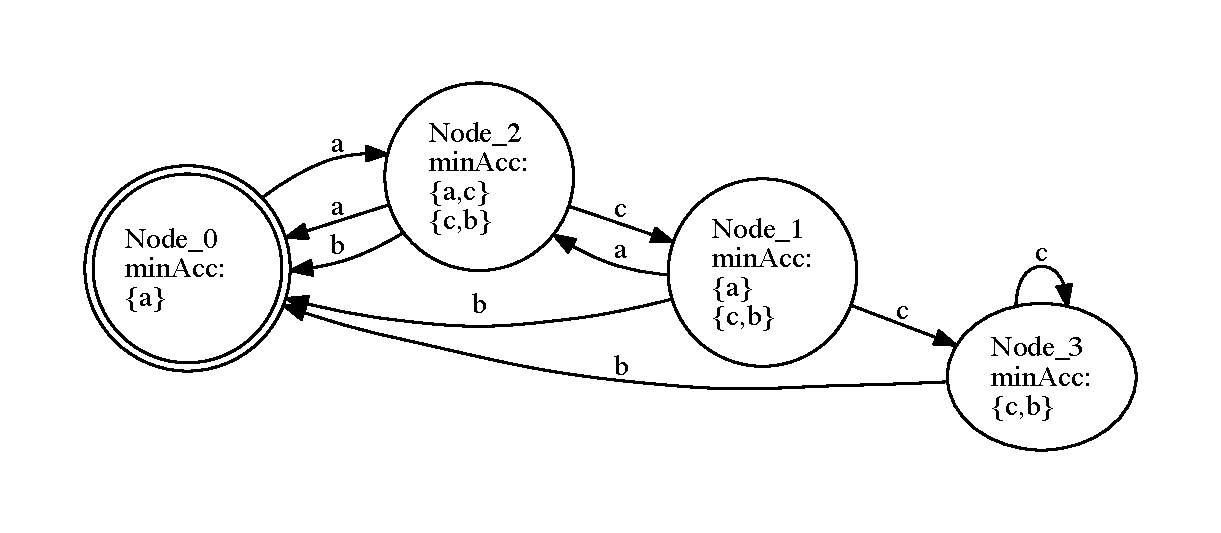
\includegraphics[width=\textwidth]{q0.pdf}
   \end{center}
   %%\vspace*{-10mm}
   \caption{Normalised transition graph of CSP process $P$ from Example~\ref{ex:a}.}
   \label{fig:tga}
 \end{figure}
% .......................................................................................

\begin{example}\label{ex:a}
We consider the process $P$ in Example~\ref{example:CSP}; its transition
graph $G(P)$ is shown in Fig.~\ref{fig:tga}. The process state
$P/\varepsilon$ (where $\varepsilon$ denotes the empty trace) is represented
as Node\_0, with $\{ a\}$ as the only minimal acceptance, since $a$ is never
refused and no other events are accepted. Having engaged in $a$, the
transition from Node\_0 leads to Node\_2 representing the process state $P/a
= Q\intchoice R$. The internal choice induces several minimal
acceptances derived from $Q$ and $R$. Since these processes accept their
initial events in external choice, $Q\intchoice R$ induces minimal acceptance
sets $\{a,c\}$ and $\{b,c\}$. Note that event $c$ can never be refused, since
it is contained in each minimal acceptance set.

Having engaged into $c$, the next process state is represented by Node\_1.
Due to normalisation, there is only a single transition satisfying
$t(\text{Node\_2},c) = \text{Node\_1}$. This transition, however, can have
been caused by either $Q$ or $R$ engaging into $c$, so Node\_1 corresponds to
process state $Q/c \intchoice R/c = P \intchoice R$. This is reflected by the
two minimal acceptance sets labelling Node\_1.
Similar considerations explain the other nodes and transitions in
Fig.~\ref{fig:tga}.

Note that the node names including their number suffixes are generated by the
FDR tool. The numbering is generated during the normalisation procedure. So,
the node numbers do not reflect the distance from the initial node Node\_0.
\xbox
\end{example}

Summarising, refinement relations between finite-state CSP processes $P, Q$ can be be
expressed by means of their normalised transition graphs
\begin{eqnarray*}
G(P) & = & ( N_P, {\ii n}_P, \Sigma, t_P : N_P\times\Sigma \pfun N_P, r_P : N_P \fun \mathbb{P}\mathbb{P}(\Sigma))
\\
G(Q) & = & ( N_Q, {\ii n}_Q, \Sigma, t_Q : N_Q\times\Sigma \pfun N_Q, r_Q : N_Q \fun \mathbb{P}\mathbb{P}(\Sigma))
\end{eqnarray*}
%
as established by results in the following lemma.
%
\begin{lemma}
  \label{lemma:tgtrcref}
  \begin{eqnarray}
  P \lessdet_T Q & \Leftrightarrow & \trc(G(Q)) \subseteq\trc(G(P))
  \label{eq:trcrefa}
  \\
  \label{eq:failconf}
  P \lessdet_F Q & \Leftrightarrow & P \lessdet_T Q \wedge P\ conf\ Q
  \\
  \label{eq:failrefa}
  P\ conf\ Q & \Leftrightarrow & \nonumber
  \forall s\in\trc(G(Q))\cap \trc(G(P)), R_Q\in r_Q(G(Q)/s):  \nonumber
  \\ & & \tabd
  \exists R_P\in r_P(G(P)/s): R_Q\subseteq R_P
  \\
  \label{eq:failrefb}
   & \Leftrightarrow &
    \forall s\in\trc(G(Q))\cap \trc(G(P)), A_Q\in\minaccs(G(Q)/s):  \nonumber
   \\ & & \tabd
  \exists A_P\in\minaccs(G(P)/s): A_P\subseteq A_Q
 \end{eqnarray}
  \xbox
\end{lemma}
%
The result (\ref{eq:trcrefa}) reflects trace refinement in terms of graph
traces; (\ref{eq:failconf}) expresses failures refinement in terms of traces
refinement and $conf$; (\ref{eq:failrefa}) states how $conf$ can be expressed
by means of the maximal refusal functions of the graphs involved; and
(\ref{eq:failrefb}) states the same in terms of the minimal acceptances that
can be derived from the maximal refusal functions by means of
(\ref{eq:maxrefsminaccs}). \fixme{alcc: I think at least the report should
point to proofs.}

% =========================================================================
\subsubsection*{Reachability Under Sets of Traces}
\label{sec:V} Given a finite-state CSP process $P$ and its normalised
transition graph $G(P)$,
%\[
%G(P) = ( N, \ii n, \Sigma, t : N\times\Sigma \pfun N, r : N \fun \mathbb{P}\mathbb{P}(\Sigma)),
%\]
suppose that $V\subseteq\Sigma^*$ is a prefix-closed set  of sequences of
events. By $t(\ii n,V)$ we denote the set
\[
t(\ii n,V) = \{ n\in N~|~\exists s\in V: s\in\trc(P)\wedge G(P)/s = n \}
\]
of nodes in $N$ that are reachable in $G(P)$ by applying traces of $V$. The
lemma below specifies a construction method for such sets $V$ reaching {\it
every} node of $N$.

\begin{lemma}
\label{lemma:extendV} Let $P$ be a CSP process with normalised transition
graph $G(P)$. %\fixme{alcc: can a
%normalised graph for a process have states that are unreachable?}
%\fxnote{jp: You are rights: all states in G(P) are reachable by construction of the graph -- I have added this information to the section introducing the graphs.}
Let
$V\subseteq\Sigma^*$ be a finite prefix-closed set of sequences of events.
Suppose that  $G(P)$ reaches $k < |N|$ nodes under $V$, that is, $|t(\ii
n,V)| = k$. Let $V.\Sigma$ denote the set of all sequences from $V$, extended
by any event of $\Sigma$. Then $G(P)$ reaches at least $(k+1)$ nodes under
$V\cup V.\Sigma$.
\end{lemma}
\begin{proof}
Suppose that $n'\in (N - t(\ii n,V))$.  Since all nodes in $N$ are reachable,
there exists a trace $s$ such that $G(P)/s = n'$. Decompose $s = s_1.e.s_2$
with $s_i\in\Sigma^*, e\in\Sigma$, such that $G(P)/s_1 \in t(\ii n,V)$ and
$G(P)/s_1.e \not\in t(\ii n,V)$. Such a decomposition always exists, because
$V$ is prefix-closed and therefore contains the empty trace $\varepsilon$.
Note, however, that it is not necessarily the case that $s_1\in V$.

Since $G(P)$ reaches $G(P)/s_1$ under $V$, there exists a trace $u\in V$ such
that $G(P)/u = G(P)/s_1 = \ol n$. Since $s = s_1.e.s_2$ is a trace of $P$ and
$G(P)/s_1 = \ol n$, then $(\ol n,e)$ is in the domain of $t$. So, $ G(P)/u.e
= G(P)/s_1.e = n$ is a well-defined node of $N$ not contained in $t(\ii
n,V)$. Since $u.e\in V\cup V.\Sigma$, $G(P)$ reaches at least the additional
node $n$ under $V\cup V.\Sigma$. This completes the proof. \xbox
\end{proof}

% =========================================================================
\subsubsection*{Graph Products}
\label{sec:GP}

For proving our main theorems, it is necessary to consider the \emph{product}
of normalised transition graphs. We need this only for the investigation of
corresponding traces in reference processes and processes for SUTs. So, the
labelling of nodes with maximal refusals or minimal acceptances are
disregarded in the product construction. We consider two normalised
transition graphs
\[
G_i = ( N_i, \ii n_i, \Sigma, t_i : N_i\times\Sigma \pfun N_i, r_i : N_i \fun \mathbb{P}\mathbb{P}(\Sigma)),\qquad i = 1,2,
\]
over the same alphabet $\Sigma$. Their product is defined by
%
\begin{eqnarray}
G_1\times G_2 & = & (N_1\times N_2,(\ii n_1,\ii n_2), t:(N_1\times N_2)\times\Sigma\pfun (N_1\times N_2))
\\
\dom~t & = & \{ ((n_1,n_2),e)\in (N_1\times N_2)\times\Sigma~|   \nonumber
\\ & & \tabc
(n_1,e)\in\dom~t_1\wedge
(n_2,e) \in\dom~t_2    \}
\\
t((n_1,n_2),e) & = & (t_1(n_1,e),t_2(n_2,e))\ \text{for $((n_1,n_2),e)\in\dom~t$}
\end{eqnarray}
%
The following lemma is used in the proof of our main theorem.
%
\begin{lemma}\label{lemma:reachproduc}
If $G_1$ has $p$ states and $G_2$ has $q$ states, then every reachable state
$(n_1,n_2)$ of the product graph $G_1\times G_2$ can be reached by a trace
%%%$s\in\trc(G_1)\cap \trc(G_2)$  we don't need this
of maximal length $(pq-1)$.
\end{lemma}
\begin{proof}
The product graph $G_1\times G_2$ has at most $pq$ states. The empty trace $\varepsilon$
reaches its initial state $(\ii n_1,\ii n_2)$. Applying Lemma~\ref{lemma:extendV}
$(pq-1)$ times with $V=\{\varepsilon \}$ implies that $G_1\times G_2$ reaches
all of its reachable states (there are at most $pq$ of them) under
$V' = V \cup V.\Sigma\cup\dots \cup V.\Sigma^{(pq-1)}$. The maximal length of traces in
$V'$ is $(pq-1)$.
\xbox
\end{proof}


% =========================================================================
\subsection{Minimal Hitting Sets}
\label{sec:hit}
% =========================================================================

The main idea of the underlying test strategy for failures refinement can be
based on solving a \emph{hitting set problem}. Given a finite collection of
finite sets $C = \{ A_1,\dots,A_n\}$, such that each $A_i$ is a subset of a
universe $\Sigma$, a \emph{hitting set} $H\subseteq\Sigma$ is a set
satisfying the following property.
%
\begin{equation}
  \label{eq:hit}
  \forall A\in C: H\cap A \neq\varnothing.
\end{equation}
%
A \emph{minimal hitting set} is a hitting set that cannot be further reduced
without losing the characteristic property (\ref{eq:hit}). By $\minhits(C)$
we denote the collection of minimal hitting sets for a collection $C$. For
the pathological case where $C$ contains an empty set, $\minhits(C)$ is also
empty.

The problem of determining minimal hitting sets is %%% \cite{Book1975-BOOKRM,5533149}
NP-hard~\cite{5533149}. We see below, however, that it reduces the effort of
testing for failures refinement from a factor of $2^{|\Sigma|}$ to a factor
that equals the number of minimal hitting sets.

The following lemma establishes that the $conf$ relation specified in
(\ref{eq:conf}) can be characterised by means of minimal acceptances and
their minimal hitting sets.
%
\begin{lemma}
\label{lemma:hseta}
Let $P, Q$ be two finite-state CSP processes.
%% satisfying $P\lessdet_T Q$.
For each $s\in\trc(P)$,
let $\minhits(P/s)$ denote the
collection of all minimal hitting sets of $\minaccs(P/s)$.
Then the following statements are equivalent.
\begin{enumerate}
\item $P\ conf\ Q$

\item For all $s\in\trc(P)\cap \trc(Q)$ and $H \in  \minhits(P/s)$, $H$ is
a (not necessariliy minimal) hitting set of $\minaccs(Q/s)$.
\end{enumerate}
\end{lemma}
\begin{proof}
For showing ``$1 \Rightarrow 2$'', assume   $P\ conf\ Q$ and
  $s\in\trc(P)\cap \trc(Q)$. Lemma~\ref{lemma:tgtrcref},
(\ref{eq:failrefb}), states that
\[
\forall A_Q\in\minaccs(G(Q)/s):
\exists A_P\in\minaccs(G(P)/s): A_P\subseteq A_Q
\]
Therefore, $H \in  \minhits(P/s)$ not only implies $H\cap A_P\neq\varnothing$
for all minimal acceptances $A_P$, but also $H\cap A_Q\neq\varnothing$ for
every minimal acceptance $A_Q$, because $A_P\subseteq A_Q$ for at least one
$A_P$. As a consequence, each $H \in \minhits(P/s)$ is also a hitting set for
$\minaccs(G(Q)/s)$ as required.

To prove ``$2 \Rightarrow 1$'', assume that 2 holds, but that $P\ conf\ Q$
does {\it not} hold. According to Lemma~\ref{lemma:tgtrcref},
(\ref{eq:failrefb}), there exists $s\in\trc(P)\cap \trc(Q)$ such that
\[
\exists A_Q\in\minaccs(G(Q)/s): \forall A_P\in\minaccs(G(P)/s): A_P\not\subseteq A_Q
\qquad (*)
\]
Let $A$ be such an acceptance set $A_Q$ fulfilling (*).
Define
\[
\overline H = \bigcup\{ A_P \setminus A~|~A_P\in\minaccs(G(P)/s) \}.
\]
Since $A_P \setminus A \neq\varnothing$ for all $A_P$ because of (*),
$\overline H$ is a hitting set of $\minaccs(G(P)/s)$ which has an  empty
intersection with $A$.
Minimising $\overline H$ yields   a minimal hitting set $H\in
\minhits(P/s)$ which is {\it not} a hitting set of $\minaccs(G(Q)/s)$, a
contradiction to Assumption~2. This completes the proof of the lemma. \xbox
\end{proof}
%
We note that $\minaccs(P) = \{ \varnothing \}$ if $P = Q\intchoice \Stop$.
Since $\Stop$ accepts nothing, its minimal acceptance is $\varnothing$, and
this carries over to $Q\intchoice \Stop$.  From (\ref{eq:failrefb}) we
conclude that $\varnothing\in\minaccs(P)$ implies $\minaccs(P) = \{
\varnothing \}$. This clarifies that $\minhits(P/s)$ is empty if, and only
if, $\minaccs(P) = \{ \varnothing \}$. The proof of Lemma~\ref{lemma:hseta}
covers the situations where $\minaccs(P/s) = \{ \varnothing \}$ and so
$\minhits(P/s) = \varnothing$.


% ==========================================================================
\section{Finite Complete Test Suites for CSP Failures Refinement}
\label{sec:finitecompletefails}
% ==========================================================================

Given a finite-state CSP process $P$ and its normalised transition graph
\[
G(P) = ( N, \ii n, \Sigma, t : N\times\Sigma \pfun N, r : N \fun \mathbb{P}\mathbb{P}(\Sigma)),
\]
suppose that $V\subseteq\Sigma^*$ is a
prefix-closed set  of sequences of events. By $t(\ii n,V)$ we denote the set
\[
t(\ii n,V) = \{ n\in N~|~\exists s\in V: s\in\trc(P)\wedge G(P)/s = n \}
\]
of nodes in $N$ that are reachable in $G(P)$ by applying traces of $V$.

\begin{lemma}
\label{lemma:extendV} Let $P$ be a CSP process with normalised transition
graph $G(P)$, such that all states in $N$ are reachable. \fixme{alcc: can a
normalised graph for a process have states that are unreachable?} Let
$V\subseteq\Sigma^*$ be a finite prefix-closed set of sequences of events.
Suppose that  $G(P)$ reaches $k < |N|$ nodes under $V$, that is, $|t(\ii
n,V)| = k$. Let $V.\Sigma$ denote the set of all sequences from $V$, extended
by any event of $\Sigma$. Then $G(P)$ reaches at least $(k+1)$ nodes under
$V\cup V.\Sigma$.
\end{lemma}
\begin{proof}
Suppose that $n'\in (N - t(\ii n,V))$.  Since all nodes in $N$ are reachable,
there exists a trace $s$ such that $G(P)/s = n'$. Decompose $s = s_1.e.s_2$
with $s_i\in\Sigma^*, e\in\Sigma$, such that $G(P)/s_1 \in t(\ii n,V)$ and
$G(P)/s_1.e \not\in t(\ii n,V)$. Such a decomposition always exists, because
$V$ is prefix-closed and therefore contains the empty trace $\varepsilon$.
Note, however, that it is not necessarily the case that $s_1\in V$.

Since $G(P)$ reaches $G(P)/s_1$ under $V$, there exists a trace $u\in V$ such
that $G(P)/u = G(P)/s_1 = \ol n$. Since $s = s_1.e.s_2$ is a trace of $P$ and
$G(P)/s_1 = \ol n$, then $(\ol n,e)$ is in the domain of $t$. So, $ G(P)/u.e
= G(P)/s_1.e = n$ is a well-defined node of $N$ not contained in $t(\ii
n,V)$. Since $u.e\in V\cup V.\Sigma$, $G(P)$ reaches at least the additional
node $n$ under $V\cup V.\Sigma$. This completes the proof. \xbox
\end{proof}
\fixme{alcc: Explain the structure of the section? Can the above result be in
a section, rather than the introduction of the section?}

% ==========================================================================
\subsection{Test Cases for Verifying CSP Failures Refinement}

For a given reference process $P$ and for each integer $p\ge 0$, we define a
CSP test process for failures refinement as shown below.
%
\begin{eqnarray}
U_F(p) & = & U_F(p,\varepsilon)
\\
U_F(p,s) & = & \big( \Extchoice e:(\Sigma - [P/s]^0) @ e \then \efail\then \Stop \big)
\label{eq:ufa}
\\ & & \extchoice \nonumber
\\ & & ([P/s]^0 = \varnothing)    \&   \big( \epass \then \Stop \big)
\label{eq:ufb}
\\ & & \extchoice \nonumber
\\ & & (\#s < p) \& \big( \Extchoice e:[P/s]^0 @ e \then U_F(p,s.e) \big)
\label{eq:ufc}
\\ & & \extchoice \nonumber
\\ & & (\#s = p) \& \big( \sqcap_{H\in\text{minHit}(P/s)} ( \Extchoice e:H @ e \then \epass \then\Stop   )  \big)
\label{eq:ufd}
\end{eqnarray}
%
A test is performed by running $U_F(p)$ concurrently with any SUT process $Q$
\fixme{alcc: add an example?} that operates on the same alphabet as $P$,
synchronising over alphabet $\Sigma$. Therefore, a test execution is any
trace of the concurrent process
\[
Q\parallel[\Sigma] U_F(p).
\]
It is assumed that the events $\efail$ and $\epass$, denoting FAIL and PASS
of the test execution, are events outside $\Sigma$. Since we assume that $Q$
is free of livelocks, it is guaranteed that each test execution terminates
after some $s\in\trc(P)$ with length $(p+1)$ at the latest. The test is
\emph{passed} by the SUT (written $Q\ \pass\ U_F(p)$) if, and only if, {\it
every} execution of $Q\parallel[\Sigma] U_F(p)$ terminates with PASS event
$\epass$. This can also be  expressed by means of a failures refinement.
\[
Q\ \pass\ U_F(p) \equiv (\epass\then\Stop) \lessdet_F (Q\parallel[\Sigma] U_F(p)) \hide \Sigma
\]
This type of pass relation is often called \emph{must test}, because every
test execution must end with the $\epass$
event~\cite{Hennessy:1988:ATP:50497}. Note that it is necessary to use the
failures-refinement relation in this condition, and not the trace-refinement
relation:~$(Q\parallel[\Sigma] U_F(p)) \hide \Sigma$ may have  the same
visible traces $\varepsilon$ and $\langle \epass\rangle$ as the ``Test Passed
Process'' $(\epass\then\Stop)$. However, the former may nondeterministically
refuse $\epass$, due to a deadlock occurring when a faulty SUT process
executes concurrently with $U_F(p,s)$ executing branch (\ref{eq:ufd}),
because $\#s = p$. This is explained further in the next paragraphs.

Intuitively speaking, $U_F(p)$ is able to perform any trace $s$ of $P$, up to
a length $p$. If, after having already run through $s\in\trc(P)$ with $\#s <
p$, an event is accepted by the SUT that is outside the initials of $P/s$,
the test immediately terminates with FAIL-event $\efail$. This is handled by
the branch (\ref{eq:ufa}) of the external choice in the process $U_F(p,s)$
defined above.

If $P/s$ is the $STOP$ process, this is revealed by its initials being empty.
In this case, the test may terminate successfully (branch (\ref{eq:ufb}) of
the external choice in $U_F(p,s)$). Note that at the same time, any (illegal)
event of the alphabet is also accepted by the test in branch~(\ref{eq:ufa}).
So, if the SUT accepts an event in a state where $P/s$ is supposed to have
stopped, there exists a test execution that terminates with FAIL by choosing
the first branch of the external choice.

If the length of $s$ is still less than $p$, the test accepts any event from
the initials $[P/s]^0$ and continues recursively as $U_F(p,s.e)$ in
branch~(\ref{eq:ufc}). A test of this type is called \emph{adaptive}, because
it accepts any legal behaviour of the SUT and adapts its consecutive
behaviour to the event selected by the SUT.

After having  run successfully
through a trace of length $p$, the test changes its behaviour:
instead of offering {\it all} legal events from $[P/s]^0$ to the SUT,
it nondeterministically chooses
a minimal hitting set of $\minaccs(P/s)$ and only offers the events contained in this set.
If the SUT refuses to engage into any of these events, this reveals a violation of the
failures refinement: according to Lemma~\ref{lemma:hseta}, a conforming SUT should accept
at least one event of each minimal hitting set in $\text{minHit}(P/s)$. Therefore, the test
only terminates with success $\epass$, if such an event is accepted by the SUT.

After this informal explanation of tests representing adaptive test cases, we are ready to prove the main theorem of this paper.

\begin{theorem}\label{th:failurestest}
Let $P$ be a divergence-free CSP process over alphabet $\Sigma$
whose normalised transition graph $G(P)$ has $p$ states. Define fault domain ${\cal D}$ as
the set of all divergence-free CSP processes over alphabet $\Sigma$, whose transition graph
has at most $q$ states with $q \ge p$.
Then the test suite
\[
\TS_F = \{ U_F(k)~|~0 \le k < pq  \}
\]
is complete with respect to ${\cal F} = (P,\lessdet_F,{\cal D})$.
\end{theorem}
\begin{proof}
To prove soundness of $\TS_F$, suppose that $Q\in{\cal D} \wedge P\lessdet_F
Q$. In this case, $\trc(Q)\subseteq \trc(P)$, and Lemma~\ref{lemma:hseta}
implies that for all traces $s$ of $Q$, every $H$ in $\text{minHit}(P/s)$ is
a hitting set for $\minaccs(Q/s)$. So, when running in parallel with $Q$, any
adaptive test $U_F(p)$ will always enter the branches (\ref{eq:ufb}),
(\ref{eq:ufc}),  or (\ref{eq:ufd}) of the external choice construction for
$U_F(p,s)$. Branch (\ref{eq:ufb}) leads always to a PASS verdict, and branch
(\ref{eq:ufc}) to test continuation without a verdict. For the last branch,
we note that any selected minimal hitting set $H\in\text{minHit}(P/s)$ has a
non-empty intersection with each of the minimal acceptances of $Q/s$. As a
consequence, $Q/s$ never blocks when offered events from $H$, and the test
terminates with PASS event $\epass$. Note that this argument requires that
$Q$ is free of livelocks, because otherwise the PASS-events might not become
visible, due to unbounded sequences of hidden events performed by $Q$. Note
further, that this proof did not refer in any way to the size of $Q$'s
normalised transition graph, so the test suite is sound for {\it all}
non-divergent CSP process refining $P$. \fixme{alcc: Soundness does not
depend on the fault domain. I would have it as a separate theorem.}

To prove exhaustiveness, consider a process $Q\in{\cal D}$ with
$P\not\lessdet_F Q$. This non-conformance can be caused in two possible ways.
\begin{description}
\item[Case~1] $\trc(Q)\not\subseteq \trc(P)$
\item[Case~2] There exists a joint trace $s\in\trc(Q)\cap\trc(P)$ and a minimal acceptance $A_Q$
of $\minaccs(Q/s)$, such that
(see Lemma~\ref{lemma:tgtrcref}, (\ref{eq:failrefb})).
\begin{equation}
\label{eq:accsnotcontained}
\forall A_P\in\minaccs(P/s): A_P\not\subseteq A_Q,
\end{equation}
\end{description}
It has to be shown for each of the two possibilities that at least one test
execution of some $(Q\parallel[\Sigma] U_F(k))$ with $k < pq$ ends with the
FAIL event $\efail$ or without giving any verdict. The latter case is also
interpreted  as FAIL, since then the process $\epass\then\Stop$ is no longer
failures-refined by the test execution.

For the first case, consider a  trace $s.e\in\trc(Q)$ such that
$s\in\trc(P)$, but $s.e\not\in\trc(P)$. Such a trace always exists because
$\varepsilon$ is a trace of every process. In this case, $s$ is also a trace
of the product graph $G = G(P)\times G(Q)$ defined in Section~\ref{sec:ntg}.
From the construction of $G$ described there, we know that $G$ has at most
$pq$ reachable states, because $G(P)$ has $p$ states, and $G(Q)$ has at most
$q$ states. Suppose that $G/s = (n_P,n_Q)$. Applying
Lemma~\ref{lemma:extendV} implies that this state can be reached by a trace
$u\in\trc(G)$ of length $\#u < pq$. Now the construction of the transition
function of $G$ implies that $u$ is also a trace of $P$ and $Q$. Since test
$U_F(pq-1)$ accepts all traces of $P$ up to length $pq-1$, $u$ is also a
trace of this test, and, by construction, $U_F(pq-1)/u = U_F(pq-1,u)$. Since
$s.e\not\in\trc(P)$, $e$ is an element of $\Sigma-[P/u]^0$. Therefore, in at
least one execution, $U_F(pq-1,u)$ executes its first branch (\ref{eq:ufa})
with this event $e$, so that the test fails with event $\efail$. Again, the
assumption of non-divergence of Q is needed for this conclusion. \fixme{alcc:
I didn't see how Lemma 3 is being applied here. Also, given the definition of
the test as a process, I'm not sure why you need to make the argument using
graph product.}

For the Case~2, we note that trace $s$ is again a trace of the product graph
$G$. Therefore, $G/s$ can again be reached by a trace
$u\in\trc(Q)\cap\trc(P)$ of maximal length $\#u < pq$. Consider test $U_F(\#
u)$, which satisfies $U_F(\# u)/u = U_F(\#u,u)$, because it always performs
branch (\ref{eq:ufc}) until the trace $u$ has been completely processed.
$U_F(\#u,u)$ may execute branches (\ref{eq:ufa}) or (\ref{eq:ufd})
only:~assumption (\ref{eq:accsnotcontained}) in Case~2 implies that $P/s$ has
at least one non-empty minimal acceptance, so the guard condition $([P/s]^0 =
\varnothing)$ of branch (\ref{eq:ufb}) evaluates to $\isf$ for $U_F(\#u,u)$.
Moreover, the guard condition $(\#s < p)$ for branch (\ref{eq:ufc}) evaluates
to $\isf$ for $U_F(\#u,u)$, too. If branch (\ref{eq:ufa}) is executed, the
test always fails. If branch (\ref{eq:ufd}) is executed, the test fails for
the execution where a minimal hitting set $H\in\text{minHit}(P/u)$ is chosen
by $U_F(\#u,u)$ that has an empty intersection with the minimal acceptance
$A_Q$ from condition (\ref{eq:accsnotcontained}). The existence of such an
$H$ is guaranteed because of Lemma~\ref{lemma:hseta}. As a consequence, there
exists a test execution   where $Q/u$ selects acceptance $A_Q$ and
$U_F(\#u,u)$ selects $H$. This execution deadlocks in process state
$(Q\parallel[\Sigma]U_F(\# u))/u$, so it cannot produce the pass event
$\epass$; this  means that the test fails. This concludes the proof. \xbox
\end{proof}


















% ==========================================================================


% =======================================================================
\section{Testing for Failures Refinement -- an Example}
\label{sec:case}
% =======================================================================

Generating the test cases $U_F(p)$ specified in  (\ref{eq:UFP}) for the reference
process $P$ discussed in Example~\ref{example:CSP},
results in the   instantiations of initials, minimal hitting sets, and
transition function shown in Fig.~\ref{fig:initialsminhitstrans};
this can be directly derived from $P$'s normalised
transition graph with nodes $N =\{0,1,2,3\}$ displayed in Fig.~\ref{fig:tga}.


\begin{figure}[htbp]
\begin{center}
\begin{minipage}{0.2\textwidth}
	 \begin{eqnarray*}
{ }[0]^0 & = & \{ a \} \\
{ }[1]^0 & = & \{ a,b,c \} \\
{ }[2]^0 & = & \{ a,b,c \} \\
{ }[3]^0 & = & \{ b,c \}
\end{eqnarray*}
	\end{minipage}
	\hfill
	\begin{minipage}{0.33\textwidth}
	 \begin{eqnarray*}
\minhits(0) & = & \{ \{ a\} \} \\
\minhits(1) & = & \{ \{a,b\}, \{c\}, \} \\
\minhits(2) & = & \{  \{a,b\},  \{a,c\},\} \\
\minhits(3) & = & \{ \{ b\}, \{c\} \}
\end{eqnarray*}

	\end{minipage}
	\hfill
	\begin{minipage}{0.2\textwidth}
	 \begin{eqnarray*}
t(0,a) & = & 1 \\
t(1,a) & = & 0 \\
t(1,b) & = & 0 \\
t(1,c) & = & 2
\end{eqnarray*}
	\end{minipage}
		\hfill
	\begin{minipage}{0.2\textwidth}
	 \begin{eqnarray*}
t(2,a) & = & 1 \\
t(2,b) & = & 0 \\
t(2,c) & = & 3 \\
t(3,b) & = & 0 \\
t(3,c) &  =& 3
\end{eqnarray*}
	\end{minipage}
	
	
	
	
\caption{Initials, minimal hitting sets, and transition function of the normalised transition graph displayed in Fig.~\ref{fig:tga}.}
\label{fig:initialsminhitstrans}
\end{center}
\end{figure}




% .....................................................................................
 \begin{figure}
 %%\hspace*{-40mm}
 \begin{center}
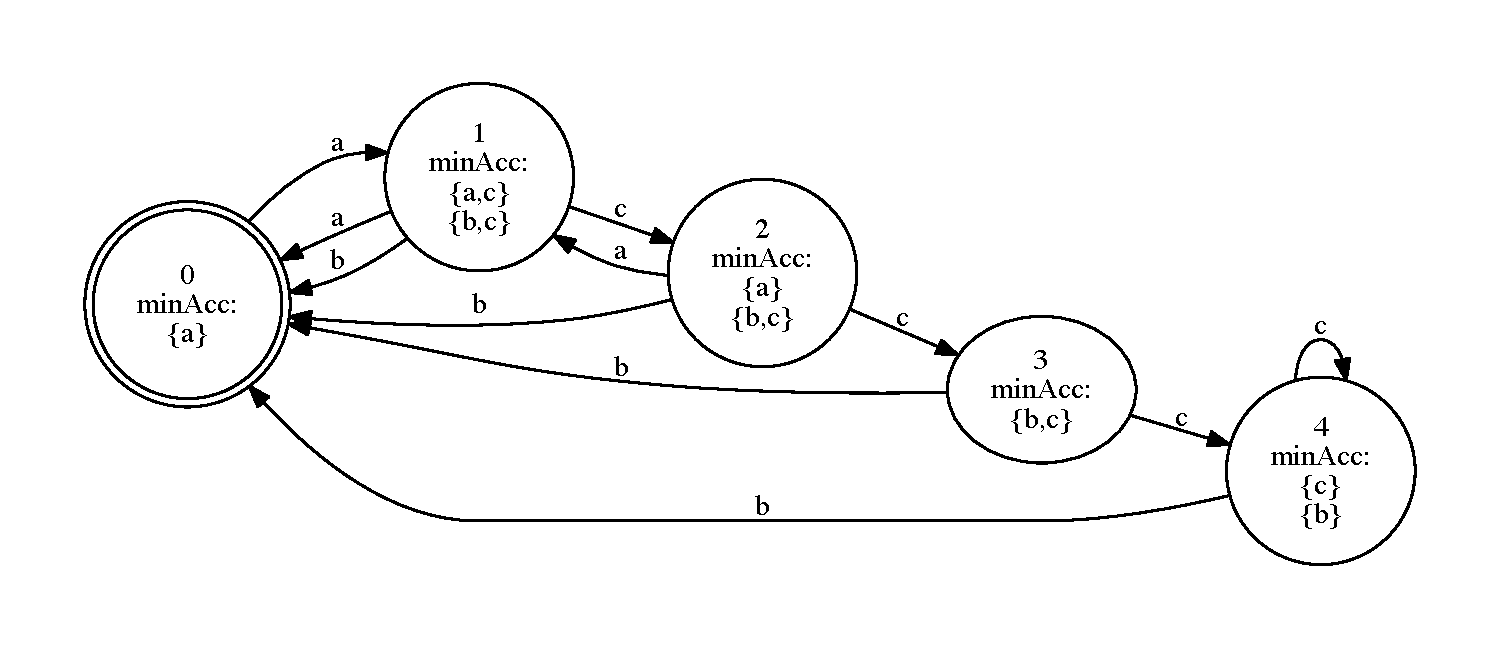
\includegraphics[width=\textwidth]{z.pdf}
\end{center}
%%\vspace*{-10mm}
\caption{Normalised transition graph of faulty implementation $Z$  from Example~\ref{ex:uf1tests}.}
 \label{fig:tgZ}
 \end{figure}
% .......................................................................................

\begin{example}
\label{ex:uf1tests} Consider the following implementation $Z$ of process $P$
from Example~\ref{example:CSP} that is erroneous from the point of view of
failures refinement. In the specification of $Z$, it is assumed that $r_{max}\ge 0$.
\begin{eqnarray*}
Z & = & a \then (Q_1 \intchoice R_1(r_{max},0))
\\
Q_1 & = & a\then Z \extchoice c\then Z
\\
R_1(r_{max},k) & = & (k < r_{max}) \& \big(b\then Z \extchoice  c\then R_1(r_{max},k+1)\big)
\\ & & \extchoice
\\ & & (k = r_{max}) \& \big(b\then Z \intchoice c\then R_1(r_{max},r_{max})\big)
\end{eqnarray*}
It is easy to see (and can be checked with FDR) that $Z$ is trace-equivalent
to $P$. While $k < r_{max}$, $Z$ also accepts the same sets of events as $P$.
When $R_1(r_{max},k)$ runs through several recursions and $k = r_{max}$,
however, $R_1(r_{max},k)$ makes an internal choice, instead of offering an
external choice, so $P\not\lessdet_F Z$. Fig.~\ref{fig:tgZ} shows the
normalised transition graph of $Z$ for $r_{max} = 3$.


Running the test $U_F(j)$ against $Z$ for $j=0,\dots,19$ ($G(P)$ has $p = 4$
states and $G(Z)$ has $q=5$, so $pq-1=19$ is the index of the last test to
be executed  according to Theorem~\ref{th:failurestest}), tests $U_F(0),\dots,
U_F(3)$ are passed by $Z$, but $Z$ fails $U_F(4)$, because after execution of
the trace
\[
s = a.c.c.c, \qquad\text{(note that $G(P)/s = \text{node}\ 3$ according to Fig.~\ref{fig:tga})},
\]
the test $U_F(4)$ offers hitting sets from $\minhits(3) = \{\{b\},\{c\}\}$
in branch (\ref{eq:ufd}). Therefore,  there exists one test execution
where $Z/s$ accepts only $\{b\}$ due to the internal choice (note
from Fig.~\ref{fig:tgZ} that
$G(Z)/s = \text{node}\ 4$), while $U_F(4)/s$
only offers $\{c\}$ in branch (\ref{eq:ufd}) or $\{ a\} = \Sigma - [3]^0$ for
branch (\ref{eq:ufa}).  As a consequence, this execution of
$(Z\parallel[\Sigma] U_F(4))/s$ deadlocks, and the $pass$ event cannot be
produced. Another failing execution arises if $Z/s$ chooses to accept only
$\{c \}$, while $U_F(4)/s$ choses to accept only $\{a,b\}$. Therefore,
\[
(\epass\then \Stop)\not\lessdet_F  (Z\parallel[\Sigma] U_F(4)) \hide\Sigma,
\]
and the test fails. \xbox
\end{example}

% ======================================================================


% ==========================================================================
\section{Finite Complete Test Suites for CSP Trace Refinement}
\label{sec:finitecomplete}
% ==========================================================================

For establishing trace refinement, the following class of adaptive test cases
are used for a given reference process $P$ and  integers $j \ge 0$. Just as
for the tests developed  in Section~\ref{sec:finitecompletefails} to verify
failures refinement, the tests for trace refinement are derived from the
reference model's transition graph
$$
G(P) = ( N, \ii n, \Sigma, t : N\times\Sigma \pfun N, r : N \fun \mathbb{P}\mathbb{P}(\Sigma)).
$$
In contrast to the tests for failures refinement~(\ref{eq:UFP}), however, we
do not need to check the SUT with respect to its acceptance of hitting sets.
Therefore, these do not occur in the specification of the test cases below.
We use the condition on acceptances $\minaccs(n) = \{ \varnothing \}$ instead
of the condition on hitting sets $\minhits(n) = \varnothing$ in branch
(\ref{eq:utb}). From (\ref{eq:minhitminaccempty}) we know that these
conditions are equivalent, but, with the use of $\minaccs(n) = \{ \varnothing
\}$, we make it unnecessary to calculate hitting sets for generating these
tests from $G(P)$.

%\begin{eqnarray}
%U_T(p) & = & U_T(p,\varepsilon)
%\\
%U_T(p,s) & = & \big(\Extchoice e:(\Sigma - [P/s]^0) @ e \then \efail\then \Stop \big)
%\label{eq:uta}
%\\ & & \extchoice \nonumber
%\\ & & (\minaccs(P/s) = \{ \varnothing \})   \&   \big( \epass \then \Stop \big)
%\label{eq:utb}
%\\ & & \extchoice \nonumber
%\\ & & (\#s < p) \& \big(\Extchoice e:[P/s]^0 @ e \then U_T(p,s.e) \big)
%\label{eq:utc}
%\\ & & \extchoice \nonumber
%\\ & & (\#s = p) \& \big( \epass\then \Stop  \big)
%\label{eq:utd}
%\end{eqnarray}

\begin{eqnarray}
U_T(j) & = & U_T(j,0,\ii n)
\\
U_T(j,k,n) & = & \big(  e:(\Sigma - [n]^0)   \then \efail\then \Stop \big)
\label{eq:uta}
\\ & & \extchoice \nonumber
\\ & & (\minaccs(n) = \{ \varnothing \})   \&   \big( \epass \then \Stop \big)
\label{eq:utb}
\\ & & \extchoice \nonumber
\\ & & (k < j) \& \big( e:[P/s]^0   \then U_T(j,k+1,t(n,e)) \big)
\label{eq:utc}
\\ & & \extchoice \nonumber
\\ & & (k = j) \& \big( \epass\then \Stop  \big)
\label{eq:utd}
\end{eqnarray}
%
It is easy to see that the tests $U_T(j)$ satisfy the properties
\begin{eqnarray}
\label{eq:ifpaT}
  &  & U_T(j)/s = U_T(j,\#s,G(P)/s)
\\
\label{eq:ifpbT}
e\not\in [P/s]^0 & \implies & U_T(j)/s.e = (\efail\then\Stop)
\end{eqnarray}
proven in Lemma~\ref{lemma:ufproperties} for $U_F(j)$ for traces
$s\in\trc(P)$ with $\#s \le j$.

%The difference between adaptive tests $U_T(p)$ for trace refinement and
%$U_F(p)$ for failures refinement consists in the fact that the former do not
%``probe'' the SUT with respect to minimal sets of events to be accepted
%without blocking.

% ==========================================================================
Since the test $U_T(j)$ never blocks any event of an SUT process $Q$ before
terminating, the pass criterion, defined below, can be based on
trace instead of failures refinement as required in (\ref{eq:passF}).
%
\begin{equation}
\label{eq:passT}
Q\ \pass\ U_T(j) \defs (\epass\then\Stop) \lessdet_T (Q\parallel[\Sigma] U_T(j)) \hide \Sigma
\end{equation}
%
If the SUT process $Q$ deadlocks after a trace $s$, and in this case the
reference process $P$ is also in a state where deadlock is possible, this is
captured by the fact that $\minaccs(n) = \{ \varnothing\}$ for $n = G(P)/s$.
Therefore, branch (\ref{eq:utb}) of a test case execution state $U_T(j,k,n)$
with $\#s = k \le j$   can be entered and the  test execution terminates with
$\epass$. If, however, $Q$ blocks after a trace $s'$ and the reference
process satisfies $\minaccs(P/s') \neq\varnothing$, branch (\ref{eq:utb})
cannot be taken, and the test execution stops without producing $\epass$ or
$\efail$. In contrast to the test for failures refinement, this is
interpreted here as a successful test execution, because unexpected blocking
of the SUT does not violate the trace-refinement relation, as long as all
traces executed by the SUT are traces of the reference process. In
particular, if neither $\epass$ nor $\efail$ is ever produced, so that
$(Q\parallel[\Sigma] U_T(j)) \hide \Sigma = \Stop$, the test passes, because
$(\epass\then\Stop) \lessdet_T \Stop$ holds.



The existence of complete, finite test suites is expressed in analogy to
Theorem~\ref{th:failurestest}. A noteworthy difference is that the complete
suite for trace refinement just needs the single adaptive test case
$U_T(pq-1)$, while failures refinement requires the execution of $\{
U_F(0),\dots,U_F(pq-1)\}$. The reason is that $U_T(pq-1)$ identifies trace
errors for all traces up to length $pq$, while $U_F(pq-1)$ only probes for
erroneous acceptances at the end of each trace of length $(pq -1)$.
%
% -------------------------------------------------------------------------
\begin{theorem}\label{th:tracetest}
Let $P$ be a non-terminating, divergence-free CSP process over alphabet $\Sigma$ whose
normalised transition graph $G(P)$ has $p$ states. Define fault domain ${\cal
D}$ as the set of all non-terminating, divergence-free CSP processes over alphabet $\Sigma$,
whose transition graph has at most $q$ states with $q \ge p$. Then the test
suite
\[
\TS_T = \{ U_T(pq-1)   \}
\]
is complete with respect to ${\cal F} = (P,\lessdet_T,{\cal D})$.
\xbox
\end{theorem}
% -------------------------------------------------------------------------
%\begin{proof}
%The theorem follows directly
%from Step~1 in the proof of Lemma~\ref{lemma:mainfsound} and
%Case~1 in the proof of Lemma~\ref{lemma:mainfexhaustive}.
%\xbox
%\end{proof}
%%
%Examples are provided after our discussion of size of the test suites.
%
As for Theorem~\ref{th:failurestest}, the proof is structured in two lemmas,
the first ensuring soundness, and the second exhaustiveness.

% ===============================================================================
\begin{lemma}\label{lemma:mainfsoundtrace}
A test suite $\TS_T$ generated from a CSP process $P$, as specified in
Theorem~\ref{th:tracetest}, is passed by every CSP process $Q$ satisfying
$P\lessdet_T Q$.
\end{lemma}
\begin{proof}
Suppose that $P\lessdet_T Q$, so that $\trc(Q)\subseteq\trc(P)$, and assume
that $s\in\trc(Q)$ with $\#s < pq$. Since $s$ is also a trace of $P$, we can
conclude
$$U_T(pq-1)/s = U_T(pq-1,\#s,G(P)/s)$$ because of (\ref{eq:ifpaT}). Now $\trc(Q)\subseteq\trc(P)$
implies $[Q/s]^0\subseteq [P/s]^0 = [G(P)/s]^0$, so $U_T(pq-1,\#s,G(P)/s)$
cannot enter branch (\ref{eq:uta}) and produce a $\efail$ event when running
in parallel with $Q$ and synchronising over $\Sigma$. Therefore, only four
options are available for the test execution    $(Q\parallel[\Sigma]
U_T(j))/s$ to continue.

\medskip
\noindent {\bf Case~1.} $Q/s$ deadlocks and $\minaccs(G(P)/s) = \{
\varnothing \}$. In this case, the test $U_T(pq-1,\#s,G(P)/s)$ enters branch
(\ref{eq:utb}), and its execution stops after $\epass$.

\medskip
\noindent {\bf Case~2.} $Q/s$ deadlocks, but
$\minaccs(G(P)/s)\neq\{\varnothing\}$. In this case, the whole test execution
deadlocks, and this means that neither a $\epass$ nor a $\efail$ event is
produced, so the test execution is passed.

\medskip
\noindent {\bf Case~3.} $Q/s$ selects an event $e\in[Q/s]^0$ and $\#s <
pq-1$. In this case, the test $U_T(pq-1)$ in state $U_T(pq-1,\#s,G(P)/s)$ can
also engage in $e$ by entering branch (\ref{eq:utc}), and its execution
continues without producing a $\epass$ or a $\efail$ event.

\medskip
\noindent {\bf Case~4.} $\#s = pq-1$ holds. In this case,
$U_T(pq-1,\#s,G(P)/s)$ can only enter branch (\ref{eq:utd}), and the test
execution stops after $\epass$.

This case analysis shows that every   execution of $(Q\parallel[\Sigma] U_T(j))$
either stops after $\epass$ or produces neither $\epass$ nor $\efail$. This
proves that $Q$ passes test $U_T(pq-1)$ according to the pass  criterion (\ref{eq:passT}).
\xbox
\end{proof}
% ===============================================================================

\begin{lemma}\label{lemma:mainfexhaustivetrace}
A test suite $\TS_T$ specified as in Theorem~\ref{th:tracetest} is
exhaustive for the fault model specified there.
\end{lemma}
\begin{proof}
As before in the proofs for failures testing, we construct the product graph
$G=G(P)\times G(Q)$ and recall that every trace $s\in\trc(P)\cap\trc(Q)$ is
associated with a path through $G$ labelled with the same events as $s$, such
that $G/s = (G(P)/s,G(Q)/s)$. Furthermore, we recall from
Lemma~\ref{lemma:extendV} that graph state $(G(P)/s,G(Q)/s)$ can always be
reached by a trace $u$ of length less or equal $pq-1$, where  the order of
$G(P)$ is $p$ and that of $G(Q)$ is $q$.

Suppose that $P\not\lessdet_T Q$. Since the empty trace is a trace of every
process, there exists a trace $s\in \trc(Q)\cap\trc(P)$ and an event $e\in
[Q/s]^0$ such that $e\not\in [P/s]^0$. Let $u\in \trc(Q)\cap\trc(P)$ be a
trace with $\#u < pq$ and $G/u = (G(P)/s,G(Q)/s)$. Then
$$
U_T(pq-1)/u = U_T(pq-1,\#u,G(P)/s).
$$
By assumption, $e\in (\Sigma -[P/s]^0) = (\Sigma - [G(P)/s]^0)$. Since
$G(Q)/u = G(Q)/s$, $Q/u$ can engage into $e$. Then $U_T(pq-1,\#u,G(P)/s)$
will enter branch (\ref{eq:uta}), and the test execution stops after having
produced $\efail$. This proves that $Q$  fails test $U_T(pq-1)$. \xbox
\end{proof}
%
Having established completeness of our test suites, we now consider the
complexity of a testing technique that uses them.


\section{Complexity Considerations}
\label{sec:complexity}
% ================================================================================

%In this section, we calculate estimates for the maximal number of test
%executions to be performed when testing for failures refinement
%and---as a corollary---trace refinement.
%Theorem~\ref{th:failurestest} specifies that all tests $U_F(j),\ 0\le j < pq$
%need to be executed, where $p$ denotes the number of nodes in the transition
%graph of the reference process $P$, and $q\ge p$ is an estimate for the
%maximal number of nodes in the SUT's transition graph. Therefore, we will first
%calculate a bound for the number of test executions to be performed for test
%$U_F(j)$ and then summarise  these bounds over all $j$ from $0$ to $pq-1$.
%
%For the worst-case estimate, we first introduce a CSP reference process $\pmax$
%which
%turns out to be--given a fixed alphabet $\Sigma$---the test
%model leading to the maximal number
%of test executions for every $U_F(j)$ when considering large alphabets. In the case
%of small alphabets and large values of $pq-1$, it will turn out below that a variant
%of $\pmax$ will lead to the maximal number of executions. The conditions for this
%can also be clearly specified.

%we assume that $P$ never allows for early
%deadlock (so $\minhits(P/s)$ is never empty) and that the SUT $Q$ is a
%correct failures refinement. Therefore, all test executions
%$(Q\parallel[\Sigma] U_F(j))$ stop after having run through a trace of $Q$ of
%length $j+1$, because their is no early termination due to entering branches
%(\ref{eq:ufa}), (\ref{eq:ufb}), or due to an illegal deadlock of $Q$. As can
%be seen from the specification of the test cases $U_F(j)$ (see
%Section~\ref{sec:finitecompletefails}), the number of executions ending in a
%$\epass$ event corresponds to the number $\ell$ of traces $s$ of $P$ with
%length equal to $j$, multiplied by the number $h$ of minimal hitting sets in
%$\minhits(P/s)$. For the tests $U_T(j)$ verifying trace refinement (see
%Section~\ref{sec:finitecomplete}), the number of executions equals $\ell$,
%since there is no equivalent in $U_T(j)$ to checking different hitting sets
%in the last step of a test execution. \fixme{But doesn't this add to the
%number of executions?} \fxnote{jp: should be clear now from the revised test}

Since we have finite complete CSP test suites, it is useful for the first
time to calculate how many test executions are needed when using them.
Previous work did not consider sufficient conditions for finiteness, so
complexity was not a concern. We answer the following questions. (1)~What is
the worst-case bound on the number of test executions to be performed to
verify an SUT with respect to failures refinement, when we use our test
suite? (2)~What is the worst-case bound for trace refinement? (3)~Is it
possible to reduce the maximal length of traces when testing for failures or
trace refinement? We consider the first question~(1) in
Section~\ref{section:complexity:failures}), where we also discuss whether it
it is possible to reduce the number of test executions with a different test
suite.  With the answer to question~(1), question~(2) is a fairly simple
consequence we discuss in Section~\ref{section:complexity:traces}.
Question~(3) is the subject of Section~\ref{section:complexity:length}.

% -------------------------------------------------------------------------
\subsection{Estimates for the Maximal Number of Failures Test Executions}
\label{section:complexity:failures}

An arbitrary CSP process $P$ might have $\minhits(P/s) = \varnothing$ for
some traces $s$, so that a test case $U_F(j)$ for a $j$ greater than the size
of $s$ can enter branch~(\ref{eq:ufb}). In this case, further executions are
needed to consider traces that have $s$ as a prefix.  To provide a bound on
the number of test executions needed, we first define a process $\pmax$~(see
(\ref{eq:pmax})), which, when used as a reference process, requires the
maximal number of test executions among all reference processes $P$
fulfilling $\minhits(P/s) != \varnothing$ for all traces $s$. For $\pmax$, we
can establish the actual number of test executions required~(see
(\ref{eq:pmaxcomplexity})).

% -----------------------------------------------------------------------------
\paragraph{A Reference Process} Given an alphabet $\Sigma$ of size $\card{\Sigma} =
n\ge 2$, define a collection of subsets of $\Sigma$ by
\begin{equation}\label{eq:defC}
  {\cal C} = \{ A\subseteq\Sigma~|~\card{A} = n - \lfloor\frac{n}{2}\rfloor + 1 \}.
\end{equation}
%
With this choice of ${\cal C}$, define
\begin{equation}\label{eq:pmax}
  \pmax = \Intchoice_{A\in{\cal C}} e:A\then \pmax
\end{equation}
%
The relevant properties of $\pmax$ are summarised in the following lemma.
%
\begin{lemma}\label{lemma:pmax}
  Given alphabet $\Sigma$ with cardinality $\card{\Sigma} = n\ge 2$,
  process $\pmax$ fulfils
  %
  \begin{eqnarray}
  {}[\pmax/s]^0 & = & \Sigma \quad\text{for all $s\in \Sigma^*$}
  \label{eq:pmaxa}
  \\
  \trc(\pmax) & = & \Sigma^*
  \label{eq:pmaxb}
  \\
  \minaccs(P/s) & = & {\cal C} \quad\text{for all $s\in \Sigma^*$}
  \label{eq:pmaxc}
  \\
  \minhits(P/s) & = & \minhits({\cal C}) \quad\text{for all $s\in \Sigma^*$}
  \label{eq:pmaxe}
  \\
  \card{\minhits(P/s)} & = & \binom{n}{\lfloor\frac{n}{2}\rfloor}
  \quad \text{for all $s\in \Sigma^*$}
  \label{eq:pmaxd}
  \\
  \minhits({\cal C})  & = & \{ H\subseteq \Sigma~|~\card{H} = \lfloor\frac{n}{2}\rfloor\}
  \label{eq:pmaxf}
  \end{eqnarray}
\end{lemma}
\begin{proof}
Since $\bigcup_{A\in{\cal C}} A = \Sigma $ by construction of ${\cal C}$,
$[\pmax]^0 = \Sigma$ and stated by (\ref{eq:pmaxa}). Since $\pmax/e = \pmax$
for all $e\in\Sigma$, this proves statement (\ref{eq:pmaxb}). The internal
choice construct used in the specification of $\pmax$ implies
$\minaccs(\pmax) = {\cal C}$. Again, $\pmax/e = \pmax$ for all $e\in\Sigma$
implies $\minaccs(\pmax/s) = {\cal C}$ for all traces of $\pmax$, so this
shows (\ref{eq:pmaxc}). Statement (\ref{eq:pmaxe}) is a direct consequence of
(\ref{eq:pmaxc}). Let $H$ be any minimal hitting set of ${\cal C}$. Then $H$
contains at least $\lfloor{\frac{n}{2}}\rfloor$ elements, because otherwise
$\card{\Sigma\setminus H} > n-\lfloor{\frac{n}{2}}\rfloor$, and any subset
$A\subseteq \Sigma\setminus H$ with cardinality
$n-\lfloor{\frac{n}{2}}\rfloor+1$  would be contained in ${\cal C}$, but
satisfy $A\cap H=\varnothing$. Since
$\lfloor{\frac{n}{2}}\rfloor+n-\lfloor{\frac{n}{2}}\rfloor+1=n+1$, we
conclude that any $\lfloor{\frac{n}{2}}\rfloor$-element subset of $\Sigma$
intersects  every element of ${\cal C}$.  Therefore, every minimal hitting
set of ${\cal C}$ has exactly $\lfloor{\frac{n}{2}}\rfloor$ elements; this
shows (\ref{eq:pmaxf}) and $\card{\minhits({\cal C})} =
\binom{n}{\lfloor{\frac{n}{2}}\rfloor}$. The latter shows  (\ref{eq:pmaxd})
and completes the proof. \xbox
\end{proof}

% -----------------------------------------------------------------------------
\paragraph{Test Cases of $\pmax$} The test cases $U_F(j)$ generated from $\pmax$ can
never enter branch (\ref{eq:ufa}), because $\pmax/s$ has initials $\Sigma$
for all traces $s\in\trc(\pmax)$ according to (\ref{eq:pmaxa}). Moreover,
they can never enter branch (\ref{eq:ufb}), because $\minhits(\pmax/s)$ is
never empty according to (\ref{eq:pmaxd}). Finally, the minimal hitting sets
used to probe the SUT at the end of a non-blocking test execution are always
the hitting sets of ${\cal C}$ according to (\ref{eq:pmaxe}). This results in
the following test case structure.
\begin{eqnarray*}
\label{eq:UFPpmax}
U_F(j) & = & U_F(j,0,\ii n)
\\
U_F(j,k,n) & = &   (k < j) \& \big(e:\Sigma   \then U_F(j,k+1,t(n,e) \big)
\\ & & \extchoice
\\ & & (k = j) \& \big( \Intchoice_{H\in\minhits({\cal C})} (e:H   \then \epass \then\Stop   )  \big)
\end{eqnarray*}
This means that the branches of $U_F(j)$ that can lead to an early
termination are not feasible. All tests deadlock, or run to the end of a
trace of size $j$ and then present the choice of event of a minimal hitting
set.

% -----------------------------------------------------------------------------
\paragraph{Maximal Number of Test Executions for $\pmax$}
When considering the number of test executions to be performed using $U_F(j)$
derived from $\pmax$ against some SUT $Q$ for all $j = 0,\dots,pq-1$, and
considering that we need to cover all the possible behaviours of $Q$, the
maximal number of test executions is only reached if (a)~$Q$ is a correct
refinement of $\pmax$ (or more generally, of the reference process) and
(b)~its traces are $\Sigma^*$.
%or if it fails in the very last execution of the very last $U_F(j)$
%executed against $Q$. If an erroneous behaviour of $Q$ is revealed before
%this very last execution, the test experiment is stopped (and $Q$ can be
%fixed before executing the suite again). Therefore, we consider only correct
%SUTs $Q$ when determining the maximal number of executions that can be
%executed.
%
%For the  $U_F(j)$ generated from $\pmax$, the number of test executions
% to be performed is maximal if $\pmax\lessdet_F Q$ and
%$\trc(Q) = \Sigma^*$.
In such a situation, no test execution blocks early, because $Q/s$ can always
engage into some $e\in\Sigma$  while $\#s<j$, and never blocks in the last
step when $\#s = j$ and a hitting set $H\in\minhits({\cal C})$ is offered by
the test case. The resulting number of executions in this case is
%
\begin{equation}
\label{eq:maxexec}
n^{j}\cdot \binom{n}{\lfloor\frac{n}{2}\rfloor},
\end{equation}
%
because \pagebreak all traces up to length $j$ can be executed with $U_F(j)$
entering branch (\ref{eq:ufc}), and each of these traces is followed by one
event from each of the hitting sets of ${\cal C}$ since $Q$ is correct.  %(b) leads to the maximal number of
%executions possible, because it is responsible for the factor *n^{(pq-1)} in
%the upper bound (47), (48) [n = |Sigma|]. Considering a reference process
%with fewer traces or an implementation Q with fewer traces would
%significantly reduce the value of this factor, while just adding one
%additional execution possibility for branch (20), after which the test suite
%is stopped due to failure.

The number of executions in (\ref{eq:maxexec}) is indeed maximal for all
reference processes $P$ fulfilling $\minhits(P/s)\neq\varnothing$ for all
traces $s$. All these processes can never enter branch (\ref{eq:ufb}), and,
if an execution with an SUT entered branch (\ref{eq:ufa}), this would only
lead to early termination of the whole test suite, because a failure has been
detected. As a consequence, $\card{\Sigma}^{j}$ is the maximal number of
traces to be executed up to length $j$, and from Theorem~\ref{th:sperner} we
know that the number $\binom{n}{\lfloor\frac{n}{2}\rfloor}$ of hitting sets
to be tested at the end of each trace of length $j$ is already maximal.

Summing up  formula (\ref{eq:maxexec}) over all test cases
$U_F(0),\dots,U_F(pq-1)$ to be executed and applying the formula for the sum
of a geometric progression,  this results int
%
\begin{equation}\label{eq:pmaxcomplexity}
\sum_{j=0}^{pq-1} n^{j}\cdot \binom{n}{\lfloor\frac{n}{2}\rfloor}  =
\binom{n}{\lfloor\frac{n}{2}\rfloor}\cdot\frac{1-n^{pq}}{1-n}\quad\text{with $n=\card{\Sigma}$}
\end{equation}
%
as the maximal number of test executions to be performed when testing an
error-free SUT $Q$ with $\trc(Q) = \Sigma^*$ against the reference process
$\pmax$. If we are interested only in the order of magnitude, the maximal
number of executions may be given as
%
\begin{equation}
\label{eq:maxO}
O\big(\binom{n}{\lfloor\frac{n}{2}\rfloor}\cdot n^{pq-1}\big)\quad\text{with $n=\card{\Sigma}$}.
\end{equation}

% -----------------------------------------------------------------------------
\paragraph{Considering Empty Collections of Minimal Hitting Sets}
The argument so far has shown that the tests derived from the reference
process $\pmax$ require the most test executions when compared to tests
derived from any other CSP process $P$ whose collections of minimal hitting
sets $\minhits(P/s)$ are never empty for any trace $s$, so that the branch
(\ref{eq:ufb}) of the related test cases $U_F(j)$ can never be entered.
Lemma~\ref{lemma:failureshittingsets} implies that an empty collection
$\minhits(P/s)$ is equivalent to $(s,A)\in\fails(P)$ for all
$A\subseteq\Sigma$. This is equivalent to $\maxrefs(P/s) = \{ \Sigma \}$ or
$\minaccs(P/s) = \{ \varnothing\}$.

It remains to consider whether reference processes $Z$ possessing failures
$(s,\Sigma)$ may require more test executions for their associated tests
$U_F(j)$ than the bound given for $\pmax$ in (\ref{eq:pmaxcomplexity}),
because process states $Z/s$ with $\minhits(Z/s)=\varnothing$ allow for test
executions entering branch (\ref{eq:ufb}). To this end, consider a test case
$U_F(j)$ constructed from such a process $Z$. Every trace $s\in\trc(Z)$ with
$\#s<j$ ending in a process state $Z/s$ with $\minhits(Z/s)=\varnothing$
allows for
%
\begin{itemize}
\item one execution of branch (\ref{eq:ufb}), where the test execution
$(Z\parallel[\Sigma]U_F(j))/s$ stops after $\epass$, and
\item $\card{[Z/s]^0}$   continuations of the test execution with events $e\in [Z/s]^0$.
\end{itemize}
%
For every trace $s\in\trc(Z)$ with $\#s=j$,
%
\begin{itemize}
\item one execution of branch (\ref{eq:ufb}) follows if
$\minhits(Z/s)=\varnothing$, and otherwise
\item $\card{\minhits(Z/s)}$ executions checking acceptance of minimal hitting sets.
\end{itemize}
%
For a rough estimate of the worst case upper bound suppose that
%
\begin{enumerate}
\item $[Z/s]^0 = \Sigma$ for all traces $s$ of $Z$,
\item all traces $s$ with $\#s<j$ end in a state with empty minimal hitting sets, and
\item all traces $s$ with $\#s=j$ end in a state with a maximal number $\binom{n}{\lfloor n/2\rfloor}$
 of hitting sets.
\end{enumerate}
%
Note that this situation cannot be realised for all $j\in\{0,\dots,pq-1\}$, because
the traces of
$U_F(p-1)$ already cover all states of $Z$'s transition graph according to Lemma~\ref{lemma:extendV}, and if all states of $Z$ have empty hitting sets, there are no acceptance checks to be performed in the last step of the test execution. Therefore, the   upper bound calculated next cannot be reached by a real CSP process.
With the 3 assumptions above, we calculate that
%
\begin{itemize}
\item  $U_F(0)$ has  $\binom{n}{\lfloor n/2\rfloor}$ executions,
\item $U_F(j),\ j > 0$ has $\sum_{i=0}^{j-1} n^i = \frac{n^j - 1}{n-1}$ executions of branch (\ref{eq:ufb}), ($n = \card{\Sigma}$), and
\item $U_F(j),\ j > 0$ has $\binom{n}{\lfloor n/2\rfloor}\cdot n^j$ executions where the acceptance of
hitting sets is checked after having run through a trace of length $j$.
\end{itemize}
%
Summing up over all $U_F(j)$ for $j=0,\dots,pq-1$,  an upper bound $B$ for the number of test executions may be calculated as follows.
%
\begin{eqnarray*}
B & = & \binom{n}{\lfloor n/2\rfloor} + \sum_{j=1}^{pq-1} \frac{n^j - 1}{n-1} +
\sum_{j=1}^{pq-1}\binom{n}{\lfloor n/2\rfloor}\cdot n^j
   \\
& = &    \sum_{j=1}^{pq-1} \frac{n^j - 1}{n-1} +
\sum_{j=0}^{pq-1}\binom{n}{\lfloor n/2\rfloor}\cdot n^j
\\
& = & \frac{n^{pq}-n pq+pq-1}{(n-1)^2} +
\binom{n}{\lfloor n/2\rfloor} \cdot \frac{n^{pq} - 1}{n-1}
\\
& = &
\\
& = & \frac{\binom{n}{\left\lfloor \frac{n}{2}\right\rfloor}(n-1) \left(n^{pq}-1\right) +n^{pq}-npq+pq-1}{(n-1)^2}
\end{eqnarray*}
%
Since  $B$ cannot be reached anyway,
we just calculate its order of magnitude, and this results again in $O\big(\binom{n}{\lfloor\frac{n}{2}\rfloor}  \cdot n^{pq-1}\big)$, as calculated already for $\pmax$ in (\ref{eq:maxO}).
%
Summarising these complexity calculations, this results in the following theorem.
%
\begin{theorem}
\label{th:maxexecs}
Given a process alphabet $\Sigma$, consider a fault model ${\cal F} = (P,\lessdet_F,{\cal D})$, such that
the normalised transition graph of $P$ has $p$ states, and the fault domain
${\cal D}$ contains all processes $Q$ over alphabet $\Sigma$, such that $G(Q)$ has at most
$q\ge p$ states. Then the maximal
number of test executions to be performed   using the complete test
suite $\TS_F = \{ U_F(j)~|~0 \le j < pq  \}$ created from $P$ as specified in Theorem~\ref{th:failurestest} is of order
%
\begin{equation*}
O\big(\binom{n}{\lfloor\frac{n}{2}\rfloor}\cdot n^{pq-1}\big)\quad\text{with $n=\card{\Sigma}$}.
\end{equation*}
For processes $P$ satisfying $(s,\Sigma)\not\in\fails(P)$ for all traces $s$, the reachable
precise  upper bound is given by
%
\begin{equation*}
\binom{n}{\lfloor\frac{n}{2}\rfloor}\cdot\frac{1-n^{pq}}{1-n}\quad\text{with $n=\card{\Sigma}$}.
\end{equation*}
\xbox
\end{theorem}
%


%
In~\cite{Hennessy:1988:ATP:50497}, it is suggested to test {\it every}
non-empty subset of $\Sigma$ whose events cannot be completely refused in a
given process state of the reference model; this leads to a worst-case
estimate of $2^{\card{\Sigma}}-1$ for the number of different sets to be
offered to the SUT in the last step of the test execution. This number is significantly larger than the worst-case estimate $\binom{n}{\lfloor n/2\rfloor}$ calculated above for the
hitting sets to be checked.
In Fig.~\ref{fig:minhita}, the reduction is visualised by plots of
the two functions.




In~\cite{DBLP:conf/icfem/CavalcantiG07}, the authors also use minimal hitting
sets\footnote{However, they are denoted by {\it minimal acceptances}
in~\cite{DBLP:conf/icfem/CavalcantiG07}.}, but they do not give an estimate for the number of test executions to be performed.


% .....................................................................................
 \begin{figure}
 %%\hspace*{-40mm}
 \begin{center}
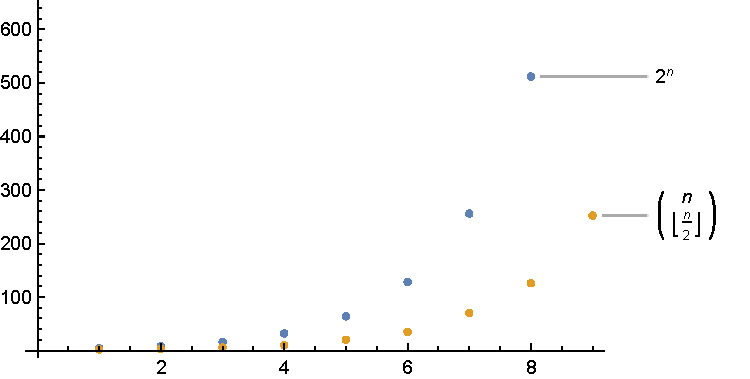
\includegraphics[width=.8\textwidth]{curvecomparison.pdf}
\end{center}
%\vspace*{-10mm}
\caption{Function plot $2^{\card{\Sigma}}$ versus $\binom{n}{\lfloor \frac{n}{2}\rfloor}$.}
 \label{fig:minhita}
 \end{figure}
% .......................................................................................


% -------------------------------------------------------------------------
\subsection{Estimates for the Maximal Number of Trace Test Executions}
\label{section:complexity:traces}

According to Theorem~\ref{th:tracetest}, a complete test suite checking trace
refinement just contains the adaptive test case $U_T(pq-1)$. As derived for
$U_F(j)$ above, the maximal number of executions to be performed by $(Q\parallel[\Sigma]
U_T(pq-1))$ is of order  $O\big(\card{\Sigma}^{pq-1}\big)$.

% -------------------------------------------------------------------------
\subsection{Upper Bound $pq$ for the Maximal Length of Test Traces}
\label{section:complexity:length}

According to Theorem~\ref{th:failurestest}, the tests $U_F(j)$ need to be
executed for $j = 0,\dots,pq-1$ to guarantee completeness.
 This means that the SUT is verified with test
traces up to, and including, length $pq$: recall from the test specification,
branch (\ref{eq:ufa}), that $U_F(j)$ will accept all traces $s.e$ with
$s\in\trc(P), \#s = j, e\not\in\trc(P/s)$, so erroneous traces up to length
$j+1$ are detected.

It is interesting to investigate whether this maximal length is really
necessary, or whether one could elaborate alternative complete test
strategies where the SUT is tested with shorter traces only. Indeed, an
example  presented in~\cite[Exercise~5]{PeleskaHuangLectureNotesMBT} shows
that when testing for equivalence of deterministic FSMs, it is sufficient to
test the SUT with traces of significantly shorter length.

The following example, however, shows that the maximal length $pq$ is really
required when testing for refinement.
%\begin{example}\label{ex:pq}
%Consider the CSP reference process $P$ and an erroneous implementation $Q$
%specified as follows.
%
%\begin{center}
%\begin{minipage}{.4\textwidth}
%\begin{eqnarray*}
%P & = & a \then P_1 \intchoice b \then P_1 \intchoice c \then P_1
%\\
%P_1 & = & a \then P \extchoice b\then P
%\end{eqnarray*}
%\end{minipage}
%\hfill
%\begin{minipage}{.4\textwidth}
%\begin{eqnarray*}
%Q & = & a\then Q_1 \extchoice b\then Q_1
%\\
%Q_1 & = & a\then Q_2 \extchoice b\then Q_2
%\\
%Q_2 & = & a\then Q \intchoice b\then Q
%\end{eqnarray*}
%\end{minipage}
%\end{center}
%
%
%\medskip
%Obviously, $P$'s normalised transition graph has 2 nodes, while $Q$'s graph
%has 3. It is easy to see (and can be checked with FDR4) that $P\lessdet_T Q$,
%but $\neg(P\lessdet_F Q)$. Furthermore, it can also be shown using FDR4 that
%the ``test passed condition''
%\[
%(\epass\then\Stop) \lessdet_F (Q\parallel[\Sigma] U_F(j))\hide \Sigma
%\]
%holds for $U_F(0),\dots,U_F(4)$, but fails for $U_F(5)$. So, the
%non-conformance of $Q$ cannot be detected by any test trace of length less or
%equal to 5, but is revealed (as expected from Theorem~\ref{th:failurestest})
%by a trace of length 6, because the last event offered by the test $U_F(5)$
%is refused by $Q$. \xbox
%\end{example}

\begin{figure}[htbp]
\begin{center}
\begin{minipage}{.4\textwidth}
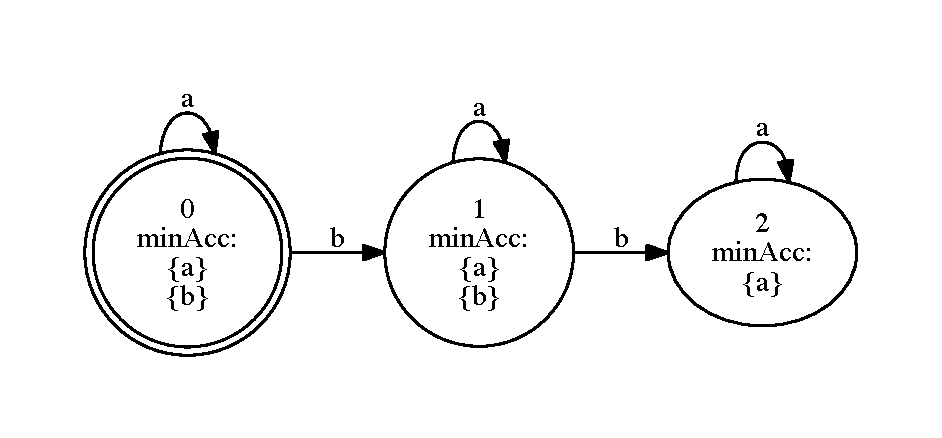
\includegraphics[width=1.2\textwidth]{theorem5p.pdf}
\end{minipage}
\hfill
\begin{minipage}{.55\textwidth}
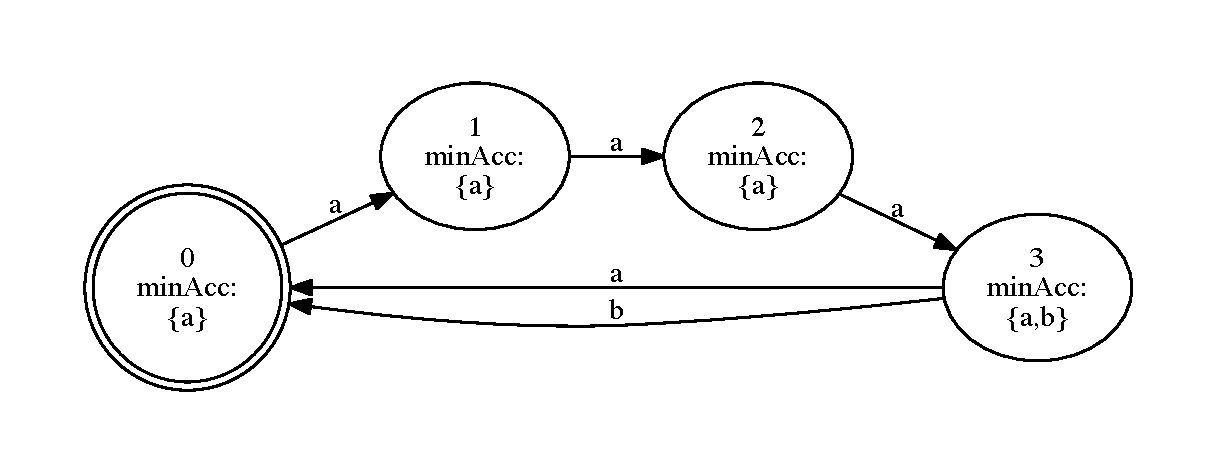
\includegraphics[width=1.2\textwidth]{theorem5q.pdf}
\end{minipage}
\caption{Transition graphs of $P$ (left) and $Q$ (right) from Example~\ref{ex:pq}
 for $p=3$ and $q=4$.}
\label{fig:examplepq}
\end{center}
\end{figure}

\begin{example}\label{ex:pq}
Consider the CSP reference process $P$ and an erroneous implementation $Q$
specified as follows.
%
\begin{eqnarray*}
P & = &  P(0)
\\
P(k) & = & (k < p-1) \& \big( (a \then P(k)) \intchoice ( b \then P(k+1))\big)
\\ & & \extchoice
\\ & & (k = p-1) \& (a \then P(k))
\\
Q & = & Q(0)
\\
Q(k) & = & (k < q-1) \& \big( a \then Q(k+1)    \big)
\\ & & \extchoice
\\ & & ( k = q-1)\& \big( a\then Q(0) \extchoice b\then Q(0)  \big)
\end{eqnarray*}
%
The normalised transition graphs of $P$ and $Q$ are depicted in
Fig.~\ref{fig:examplepq} for the case $p=3,\ q=4$. Using FDR4, it can be
shown for concrete values of $p$ and $q$ that the  ``test passed conditions''
\[
(\epass\then\Stop) \lessdet_F (Q\parallel[\Sigma] U_F(j))\hide \Sigma
\]
and
\[
(\epass\then\Stop) \lessdet_T (Q\parallel[\Sigma] U_T(j))\hide \Sigma
\]
hold for $j = 0,\dots,pq-2$. This means that none of the test cases $U_F(j)$
and $U_T(j)$ are capable of detecting failures and trace refinement
violations, if they only check traces up to length $pq-1$
(recall that this corresponds to $j\le pq-2$).

Process $Q$, however, neither conforms to $P$ in the failures refinement
relation, nor in the trace
refinement relation. This can only be seen when executing the test $U_F(pq-1)$ and
$U_T(pq-1)$, respectively. These tests fail, so this shows that $P\not\lessdet_F Q$ and
$P\not\lessdet_T Q$ according to Theorem~\ref{th:failurestest} and Theorem~\ref{th:tracetest}. Moreover, this shows that
the maximal trace
length $pq$ to be investigated in the tests cannot be further reduced without losing
the completeness property of the test suites.
\xbox
\end{example}
%
Generalising Example~\ref{ex:pq}, it can be shown that for any pair
$2\le p,q \in\mathbb{N}$,
there exist reference processes $P$ with $p$ states
and implementation processes $Q$ with $q$ states, such that
a violation of the trace refinement property
can only be detected with a trace of length $pq$. This is proven in the following
theorem. In the proof, we use the processes $P$ and $Q$ introduced in Example~\ref{ex:pq}.

% ----------------------------------------------------------------------------
\begin{theorem}\label{th:maxtracelen}
Let $2\le p,q \in\mathbb{N}$. Then there exists a reference process $P$ and an
implementation process $Q$ with the following properties.
\begin{enumerate}
\item $G(P)$ has $p$ states.
\item $G(Q)$ has $q$ states.
\item $P\not\lessdet_T Q$, and therefore, also $P\not\lessdet_F Q$.
\item $\forall s\in\trc(Q): \#s < pq\implies s\in\trc(P)$.
\item $Q\ conf\ P$.
\end{enumerate}
As a consequence, the upper bound $pq$ for the length of traces to be tested when checking for failures refinement or trace refinement
cannot be reduced without losing the test suite's completeness property.
\end{theorem}
% ----------------------------------------------------------------------------
\begin{proof}
Given $2\le p,q \in\mathbb{N}$, define reference process $P$ and implementation process $Q$ as in Example~\ref{ex:pq}. It is trivial to see that
$G(P)$ has $p$ nodes and $G(Q)$ has $q$ nodes, so statements 1 and 2 of the theorem hold.

Using regular expression notation, the traces of $P$ can be specified as
\[
\trc(P) = \prefs\big(  (a^*b)^{p-1}a^* \big),
\]
where $\prefs(M)$ denotes the set of all prefixes of traces in $M\subseteq\Sigma^*$,
including the traces of $M$ themselves.
The traces of $Q$ can be specified by
\[
\trc(Q) = \prefs\big( (a^{q-1}(a|b))^*  \big).
\]
It is easy to see that $\trc(Q)\not\subseteq\trc(P)$; for example, the trace
$(a^{q-1}b)^p$ is in $\trc(Q)\setminus\trc(P)$, because $P$-traces may contain at most $p-1$ $b$-events. This proves statement~3 of the theorem.

Let $s \in\trc(Q)$ be any trace of length $\#s = pq-1$. Then $s$ can be represented
by $s = (a^{q-1}(a|b))^{p-1}a^{q-1} \in \prefs\big( (a^{q-1}(a|b))^*  \big)$.
Then $s$ is also an element of $\trc(P)$, because $(a^{q-1}(a|b))^{p-1}a^{q-1}$
is also contained in $\prefs\big(  (a^*b)^{p-1}a^* \big)$: this is easy to see, since
$\prefs\big(  (a^*b)^{p-1}a^* \big)$ contains all finite sequences of $a$-events,
where at most $p-1$ events $b$ have been inserted. This proves statement 4 of the theorem.

To prove statement~5, we observe that the specification of $P$ implies (the
expression $(s\cnt b)$ denotes the number of $b$-events occurring in trace $s$)
\[
\minaccs(P/s) = \left\{
\begin{array}{ll}
\{ \{a\}, \{b\} \} & \text{for all $s\in\trc(P)$ with $(s\cnt b) <p-1$.}
\\
\{ \{a\} \} & \text{for all $s\in\trc(P)$ with $(s\cnt b) = p-1$.}
\end{array}
\right.
\]
and
\[
\minaccs(Q/s) = \left\{
\begin{array}{ll}
\{ \{a\}  \} & \text{for all $s\in\trc(Q)$ with $\#s \neq 0\mod(q-1)$.}
\\
\{ \{a,b\} \} & \text{for all $s\in\trc(P)$ with $\#s = 0\mod(q-1)$.}
\end{array}
\right.
\]
As a  consequence, the minimal acceptance set $A_P = \{a\}$ which is
contained in every $\minaccs(P/s)$ fulfils $A_P \subseteq A_Q$ for
any $A_Q\in\minaccs(Q/s)$, when $s\in\trc(P)\cap \trc(Q)$. Now Lemma~\ref{lemma:tgtrcref},
(\ref{eq:failrefb}) can be applied to conclude that $Q\ conf\ P$.
\xbox
\end{proof}
%
Since Theorem~\ref{th:maxtracelen} just states that a violation of trace
refinement may remain undetected if only traces shorter than $pq$ are checked
during tests, it can also be applied to our trace refinement tests.
Therefore, test suites $\{ U_T(j) \}$ with $j<pq-1$ are not complete. It is
discussed in Section~\ref{sec:conc} how the number of test traces to be
executed by complete test suites for failures or trace refinement can still
be reduced {\it without} reducing the maximal length.

% =================================================================================


%%%\section{Related Work}
\label{sec:related}

% =================================================================================














% ================================================================================



% ==============================================================================
\section{Discussion and Conclusions}
\label{sec:conc}
% ==============================================================================

% ==============================================================================
\subsubsection*{Discussion of Further Reductions of the Test Effort}
It is known from complete testing strategies for finite state machines that
the upper bound $pq$ for the lengths of the traces used in our tests to
investigate the SUT behaviour can be reduced. It is also known from FSM
testing that it is not necessary to test {\it all} traces up to this maximal
length. Notable complete strategies supporting this fact have been presented,
for example,
in~\cite{hierons_testing_2004,DBLP:conf/forte/DorofeevaEY05,petrenko_testing_2011,simao_reducing_2012}.
From~\cite{Huang2017} it is known that complete FSM testing theories can be
translated to other formalisms, such as Extended Finite State Machines,
Kripke Structures, or CSP, resulting in likewise complete test strategies for
the latter. We intend to study translations of several promising FSM
strategies to CSP in the future. These will effectively reduce the upper
bound $\ell\le |\Sigma|^k$ introduced in Section~\ref{sec:complexity}. The
bound $h$ for the number of sets to be used in probing the SUT for illegal
deadlocks, however, cannot be further reduced, as has been established in
Lemma~\ref{lemma:hseta}.

% ==============================================================================
\subsubsection*{Discussion of Adaptive Test Cases}
The tests suggested
in~\cite{Hennessy:1988:ATP:50497,DBLP:conf/icfem/CavalcantiG07} were \emph{preset} in the
sense that the trace to be executed was pre-defined for each test. As a consequence,
the authors of~\cite{DBLP:conf/icfem/CavalcantiG07} introduced \emph{inconclusive}
as a third test result, applicable to the situations where the intended trace
of the execution was blocked, due to legal, but nondeterministic behaviour of the
SUT.

In 
\fixme{From the proofs of the main theorems, and what you say below, I
thought you did have verdicts coming from deadlock, and you simply chose not
to mark it with an inc event.} 
contrast to that, our test cases specified in
Section~\ref{sec:finitecompletefails} and \ref{sec:finitecomplete} are
adaptive. This has the advantage that test executions $(Q\parallel[\Sigma]
U_F(p))$ for failures refinement never block before the final step specified
by branch (\ref{eq:ufd}), and so we do not need inconclusive test results.
It should be noted, however, that it is
necessary for our test verdicts to recognise also deadlocks in the final test
step and interpret them as FAIL, as described in
Section~\ref{sec:finitecompletefails}. In practice, this is realised by
adding a timeout event to the testing environment which indicates deadlock
situations. For real-time systems, this is an accepted technique, because the
SUT has to respond within a pre-defined latency interval, otherwise its
behaviour is considered to be blocked and regarded as a failure.
The tests executions $(Q\parallel[\Sigma] U_T(p))$ 
\fixme{Missing hiding.}
\fxnote{jp: Here, the hiding operator is not necessary: the possible test executions are really the traces of $Q$ parallel $U_T(p)$. The hiding is only needed to specify the verdict.}  
for trace refinement never
block at all before stopping after the verdict $\epass$ or $\efail$, unless the
SUT process $Q$ has an unexpected deadlock state. 
\fxfatal{And also, if the SUT blocks, the test should block,
no?}\fxnote{jp: you are right, I changed the text here and added explanations above after the verdict explanation
in formula (\ref{eq:passT}).}
Recall from the explanations given in Section~\ref{sec:finitecomplete} that the 
blocking situation also leads to passing the test, because 
$(\epass\then \Stop)\lessdet_T (Q\parallel[\Sigma] U_T(p))\hide\Sigma$ still holds
if $(Q\parallel[\Sigma] U_T(p))\hide\Sigma$ only produces the empty trace.

The adaptive behaviour of both our test case types $U_F(p)$ and $U_T(p)$,
however, induces the obligation to check that {\it all}
possible executions have been
performed before the test can be considered as passed. Typically, it is
therefore assumed that a \emph{complete testing
assumption}~\cite{hierons_testing_2004} \fixme{I think you need this for the
failures refinement tests as well.}\fxnote{jp: yes, I re-arranged the text accordingly.} holds, which means that every possible
behaviour of the SUT is performed after a finite number of test executions.
In practice, this is realised by executing each test several times, recording
the traces that have been performed, and using hardware or software coverage
analysers to determine whether all possible test execution behaviours of the
SUT have been observed. Therefore, adaptive test cases come at the price of
having to apply some grey-box testing techniques enabling us to decide
whether all SUT behaviours have been observed.

% ==============================================================================
\subsubsection*{Discussion of Fault Domains}
As already mentioned, the work in~\cite{DBLP:conf/pts/CavalcantiS17} defines
a fault domain as the set of processes that refine a given CSP process.  In
that context, only testing for traces refinement is considered, and the
complete test suites may not be finite. So, the work presented here goes well
beyond what is achieved there. On the other hand,
\cite{DBLP:conf/pts/CavalcantiS17} presents an algorithm for test generation
that can be easily adapted to consider additional selection and termination
criteria, like, for example, the length of the traces used to construct
tests. It would be possible, for instance, to use the bound indicated here.
Moreover, specifying a fault domain as a CSP process allows us to model
domain-specific knowledge using CSP. For example, if an initialisation
component defined by a process $I$ can be regarded as correct without further
testing, we can use $I; RUN$ as a fault domain, to indicate that any SUT of
interest implements $I$ correctly, but afterwards has a potentially arbitrary
behaviour specified by $RUN$. In addition, the work
in~\cite{DBLP:conf/pts/CavalcantiS17} is not restricted to finite or
non-terminating processes.

% ==============================================================================
\subsubsection*{Implications for CSP Model Checking}
As explained in the previous sections, passing a test is specified by
$(\epass\then\Stop) \lessdet_F (Q\parallel[\Sigma] U_F(k)) \hide \Sigma$ for
failures testing. If the SUT $Q$ is not a programmed piece of software or an
integrated hardware or software system, but just another CSP process
specification, it is of course possible to verify the pass criterion using
the FDR4 model checker. For checking the refinement relation $P\lessdet_F Q$,
the pass criterion has to be verified for $k=0,\dots,pq-1$, where $p$ and $q$
indicate the number of nodes in $P$'s transition graph and the maximal number
of nodes in $Q$'s graph, respectively (Theorem~\ref{th:failurestest}). Since
the test cases $U_F(k)$ have such a simple structure, it is an interesting
question for further research whether checking $(\epass\then\Stop) \lessdet_F
(Q\parallel[\Sigma] U_F(k)) \hide \Sigma$ for $k=0,\dots,pq-1$ can be faster
than directly checking $P\lessdet_F Q$, as one would do in the usual approach
with FDR4. This is of particular interest, since the checks could be
parallelised on several CPUs. Alternatively it is interesting to investigate
whether the check\footnote{We are grateful to Bill Roscoe for suggesting this
option.}
\[
(\epass\then\Stop) \lessdet_F (Q\parallel[\Sigma] \Intchoice_{k=0}^{pq-1} U_F(k)) \hide \Sigma
\]
may perform better than the check of $P\lessdet_F Q$, since the former allows for
other optimisations in the model checker than the latter.

For large and complex CSP processes $Q$, it may be too time consuming to
generate its normalised transition graph, so that its number $q$ of nodes is
unknown. In such a case the suggested options may still be used as efficient
bug finders: use  $p$ of reference process $P$ as initial $q$-value and
increment $q$ from there, as long as each increment reveals new errors.

% ==============================================================================
\subsubsection*{Conclusion}

In this paper, we have introduced finite complete testing strategies for
model-based testing against finite, non-terminating CSP reference models. The
strategies are applicable to the conformance relations failures refinement
and trace refinement. The underlying fault domains have been defined as the
sets of CSP processes whose normalised transition graphs do not have more
than a given number of additional nodes, when compared to the transition
graph of the reference process. For these domains, finite complete test
suites are available. We have shown for the strategy to check failures
refinement that the way of probing the SUT for illegal deadlocks used in our
test cases is optimal in the sense that it is not possible to guarantee
exhaustiveness with fewer probes.

% ==============================================================================

\paragraph{Acknowledgements}
The authors would like to thank Bill Roscoe and Thomas Gibson-Robinson for
their advice on using the FDR4 model checker and for very helpful discussions
concerning the potential implications of this paper in the field of model
checking. We are
grateful to Li-Da Tong from National Sun Yat-sen University, Taiwan, for
suggesting the applicability of Sperner's Theorem in the context of the work
presented here. Moreover, we thank Adenilso Simao from the University of S{\~a}o Paulo
for several helpful suggestions. 
The work of Ana Cavalcanti is funded by the Royal Academy of
Engineering and UK EPSRC Grant EP/R025134/1.


% ===============================================================================

%%%%%%%%%%%%%%%%%%%%%%%%%%%%%%%%%%%%%%%%%%%%%%%%%%%%%%%%%%%%%%%%%%%
%%%%%%%%%%%%%%%%%%%%%%%%%%%%%%%%%%%%%%%%%%%%%%%%%%%%%%%%%%%%%%%%%%%

\bibliography{references,jp}

%%%%%%%%%%%%%%%%%%%%%%%%%%%%%%%%%%%%%%%%%%%%%%%%%%%%%%%%%%%%%%%%%%%
%%%%%%%%%%%%%%%%%%%%%%%%%%%%%%%%%%%%%%%%%%%%%%%%%%%%%%%%%%%%%%%%%%%

\end{document}

%%%%%%%%%%%%%%%%%%%%%%%%%%%%%%%%%%%%%%%%%%%%%%%%%%%%%%%%%%%%%%%%%%%
%%%%%%%%%%%%%%%%%%%%%%%%%%%%%%%%%%%%%%%%%%%%%%%%%%%%%%%%%%%%%%%%%%%
